\chapter{The Deep Underground Neutrino Experiment}
\label{chapter:dune}

\begin{chapquote}{Frank Herbert, \textit{Dune}}
	Deep in the human unconscious is a pervasive need for a logical universe that makes sense. But the real universe is always one step beyond logic.
\end{chapquote}

%\noindent
The Deep Underground Neutrino Experiment (\gls{dune}) is a next generation long-baseline neutrino oscillation experiment \cite{DUNE2020TDR1}. It will address several questions in neutrino physics, study neutrinos from astrophysical sources and search for beyond the standard model physics.

This Chapter reviews the main goals of \gls{dune}, the operating principle of the \gls{lbnf} beamline, the role that the near detector plays in the oscillation measurement, and the design of the far detector modules and their data acquisition (\gls{daq}) system.

\section{Overview}

The main physics goals of \gls{dune} are:
\begin{itemize}
	\item measure the neutrino mass hierarchy, the amount of \gls{cp} violation in the leptonic sector and the $\theta_{23}$ octant,
	\item detect rare low energy neutrino events, like neutrinos from supernova bursts, and
	\item search for proton decay and other beyond the standard model phenomena.
\end{itemize}

The design of \gls{dune} has been tailored with these goals in mind. It will consist of two neutrino detectors. A near detector (\gls{nd}) complex will be placed at Fermilab, $574~\mathrm{m}$ downstream of the neutrino production point, whereas a larger far detector (\gls{fd}) will be built in the Sandford Underground Research Facility (\gls{surf}), South Dakota, approximately $1300~\mathrm{km}$ away. Figure \ref{fig:dune} shows a simplified diagram with the various components of \gls{dune} (not to scale).

\begin{figure}[t]
	\centering
	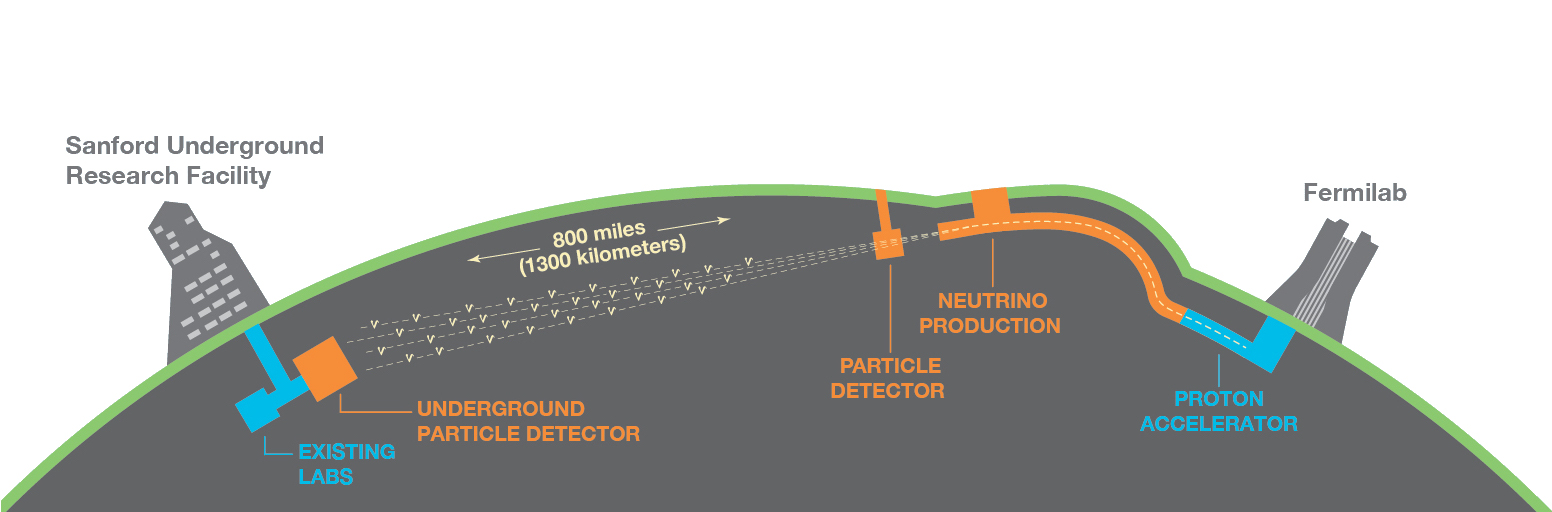
\includegraphics[width=0.9\linewidth]{Images/DUNE/FD/dune}
	\caption[Schematic diagram of the \gls{dune} experiment and the \gls{lbnf} beamline.]{Schematic diagram of the \gls{dune} experiment and the \gls{lbnf} beamline \cite{DUNE2020TDR1}.}
	\label{fig:dune}
\end{figure}

The beam neutrinos will be provided by the Long-Baseline Neutrino Facility (\gls{lbnf}) beamline, the multi-megawatt wide-band neutrino beam planned for Fermilab. It will produce neutrinos travelling in the direction of \gls{surf}, with the capability to switch between neutrino and antineutrino mode.

Before arriving to the \gls{fd}, the neutrino beam meets the \gls{nd} complex, which serves as the experiment's control. The design of the \gls{dune} \gls{nd} is mainly driven by the needs of the oscillation physics programme, as its main role is to measure the unoscillated neutrino energy spectra. From these we can predict the unoscillated spectra at the \gls{fd}, which can be compared to the spectra measured at the \gls{fd} to extract the oscillation parameters. Additionally, the \gls{nd} has a physics programme of its own, including cross section measurements and \gls{bsm} physics searches.

The technology chosen for the \gls{fd} modules of \gls{dune} is the liquid Argon time projection chamber (\gls{lartpc}). Its four modules will record neutrino interactions from the accelerator-produced beam arriving at predictable times. As it also aims to record rare and low energy events, like supernovae and solar neutrinos, the \gls{fd} requires trigger schemes which can deal with both kinds of physics, and also maximum uptime.

\begin{table}[]
	\caption[Summary of the two-phased plan for \gls{dune}.]{Summary of the two-phased plan for \gls{dune}. Adapted from Ref. \cite{DUNE2022Snowmass}.}
	\centering
	\begin{tabular}{c|C{3.0cm}|C{3.0cm}|c}
	Parameter  & Phase I                     & Phase II		& Benefit \\[1mm] \hline
	\rule{0pt}{1.1\normalbaselineskip}\gls{fd} mass    & $20 \ \mathrm{kt}$ fiducial & $40 \ \mathrm{kt}$ fiducial & \gls{fd} statistics\\[1mm]
	Beam power & up to $1.2 \ \mathrm{MW}$   & $2.4 \ \mathrm{MW}$      & \gls{fd} statistics  \\[1mm]
	\gls{nd} config.  & \gls{ndlar}, \gls{tms}, \gls{sand}           & \gls{ndlar}, \gls{ndgar}, \gls{sand} & Systematic constraints
	\end{tabular}
	\label{tab:dune_phases}
\end{table}

\gls{dune} is planned to be built using a staged approach consisting of two phases, which are summarised in Tab. \ref{tab:dune_phases}. Phase I consists of a \gls{fd} with $50\%$ of the total fiducial mass, a reduced version of the \gls{nd} complex and a $1.2~\mathrm{MW}$ proton beam. It will be sufficient to achieve some early physics goals, like the determination of the neutrino mass ordering. For its Phase II, \gls{dune} will feature the full four \gls{fd} modules, a more capable \gls{nd} and a $2.4~\mathrm{MW}$ proton beam. The physics milestones for the two phases are given in Tab. \ref{tab:dune_phases_physics}, in a staging scenario which assumes that Phase II is completed after six years of operation.

A summary of the \gls{dune} science programme can be found in the \gls{dune} \gls{fd} Technical Design Report (\gls{tdr}) Volume I \cite{DUNE2020TDR1}. For a detailed discussion on the two-phased approach the reader is referred to the \gls{dune} Snowmass 2021 report \cite{DUNE2022Snowmass}.

\section{Physics goals of DUNE}

\begin{table}[]
	\caption[Exposure and time required to achieve the different physics milestones of the two phases.]{Exposure and time required to achieve the different physics milestones of the two phases. The predictions assume a Phase II staging scenario where \gls{fd} modules 3 and 4 are deployed in years 4 and 6 and both the beam and \gls{nd} are upgraded after 6 years. Adapted from Ref. \cite{DUNE2022Snowmass}.}
	\centering
	\begin{tabular}{c|c|C{3.0cm}|C{2.0cm}}
	Stage    & Physics milestone                                          & Exposure (kt-MW-years) & Years (staged) \\[3mm] \hline
	\rule{0pt}{1.1\normalbaselineskip}Phase I  & $5\sigma$ MO ($\delta_{CP} = -\pi/2$)                      & 16                     & 1-2            \\[1mm]
			 & $5\sigma$ MO ($100\%$ of the $\delta_{CP}$ values)         & 66                     & 3-5            \\[1mm]
			 & $3\sigma$ CPV ($\delta_{CP} = -\pi/2$)                     & 100                    & 4-6            \\[1mm] \hline
			 \rule{0pt}{1.1\normalbaselineskip}Phase II & $5\sigma$ CPV ($\delta_{CP} = -\pi/2$)                     & 334                    & 7-8            \\[1mm]
			 & $\delta_{CP}$ resolution of $10$ degrees ($\delta_{CP}=0$) & 400                    & 8-9            \\[1mm]
			 & $5\sigma$ CPV ($50\%$ of the $\delta_{CP}$ values)         & 646                    & 11             \\[1mm]
			 & $3\sigma$ CPV ($75\%$ of the $\delta_{CP}$ values)         & 936                    & 14             \\[1mm]
			 & $\mathrm{sin}^{2}(2\theta_{13})$ resolution of $0.004$       & 1079                   & 16            
	\end{tabular}
	\label{tab:dune_phases_physics}
\end{table}

As noted in the literature (see for instance Ref. \cite{deSalas2020} for a review), the parameter space of the neutrino oscillation phenomena within the three-flavour picture is quite constrained by current experimental data. However, there are still crucial open questions, like the mass ordering, the value of $\delta_{CP}$ or the $\theta_{23}$ octant. One of the main goals of \gls{dune} is to determine precisely the values of these parameters \cite{DUNE2020TDR2}.

To address these questions \gls{dune} can look to the subdominant oscillation channel $\nu_{\mu} \rightarrow \nu_{e}$ ($\bar{\nu}_{\mu} \rightarrow \bar{\nu}_{e}$) and study the energy dependence of the $\nu_{e}$ ($\bar{\nu}_{e}$) appearance probability. When we focus on the antineutrino channel $\bar{\nu}_{\mu} \rightarrow \bar{\nu}_{e}$ there is a change in the sign of $\delta_{CP}$, thus introducing \gls{cp}-violation. Moreover, due to the absence of positrons in the composition of the Earth, there is a sign difference for the matter effect contribution when looking at the antineutrino channel. This asymmetry is proportional to the baseline length $L$ and is sensitive to the sign of $\Delta m^{2}_{31}$, and thus to the neutrino mass ordering.

Another of the main physics goals of \gls{dune} is the search for baryon-number violating processes. Specifically, it will try to answer the question of whether protons are stable or not. There is no symmetry argument that forbids protons from decaying, but its apparent stability seems to suggest that baryon number is conserved \cite{Super-Kamiokande2009}. However, proton decay is a usual feature of grand-unified theories, where electromagnetic, weak and strong interactions are unified above a certain energy scale \cite{Raby2006}.

As the energy deposition scale for these kinds of searches is nearly the same as that for long-baseline neutrino oscillations, \gls{dune} will be able to look for them. It has several advantages over other experiments, such as excellent imaging and particle identification, which can be translated into lower backgrounds.

The last of the main objectives of \gls{dune} is the detection of neutrinos originated in supernovae explosions, what is called a supernova neutrino burst (\gls{snb}). These neutrinos carry with them information about the core-collapse process, from the progenitor to the explosion and the remnant; but also may have information about new exotic physics. So far, the only neutrino events ever recorded from such a process were a few dozens of $\bar{\nu}_{e}$ events from the 1987A supernova located in the Magellanic Cloud, $50~\mathrm{kpc}$ away from Earth \cite{Kamiokande-II1987, Bionta1987}.

\gls{dune} aims to collect \gls{snb} events. Although these are quite rare, as the expected supernovae explosion events are about one every few decades for our galaxy and Andromeda, the long lifetime of the experiment (around a couple of decades as well) makes it reasonable to expect some. Nowadays the main sensitivity to \gls{snb} of most experiments is via the $\bar{\nu}_{e}$ flux from inverse beta decay. One of the advantages of \gls{dune} is its expected sensitivity to MeV-scale $\nu_{e}$ events, since the dominant channel will be $\nu_{e}$ \gls{cc} scattering.

Moreover, due to the stringent requirements that the main physics goals set for \gls{dune}, it will also enable searches for all kind of \gls{bsm} physics. Among other things, \gls{dune} will be able to look for: active-sterile neutrino mixing, non-unitarity of the \gls{pmns} matrix, non-standard interactions, Lorentz and \gls{cpt} violations, neutrino trident production, light-mass \gls{dm}, boosted \gls{dm}, and heavy neutral leptons. The reader is referred to the \gls{dune} \gls{fd} \gls{tdr} Volume II \cite{DUNE2020TDR2} for a full discussion of the physics scope of \gls{dune}.

\begin{figure}[t]
	\centering
	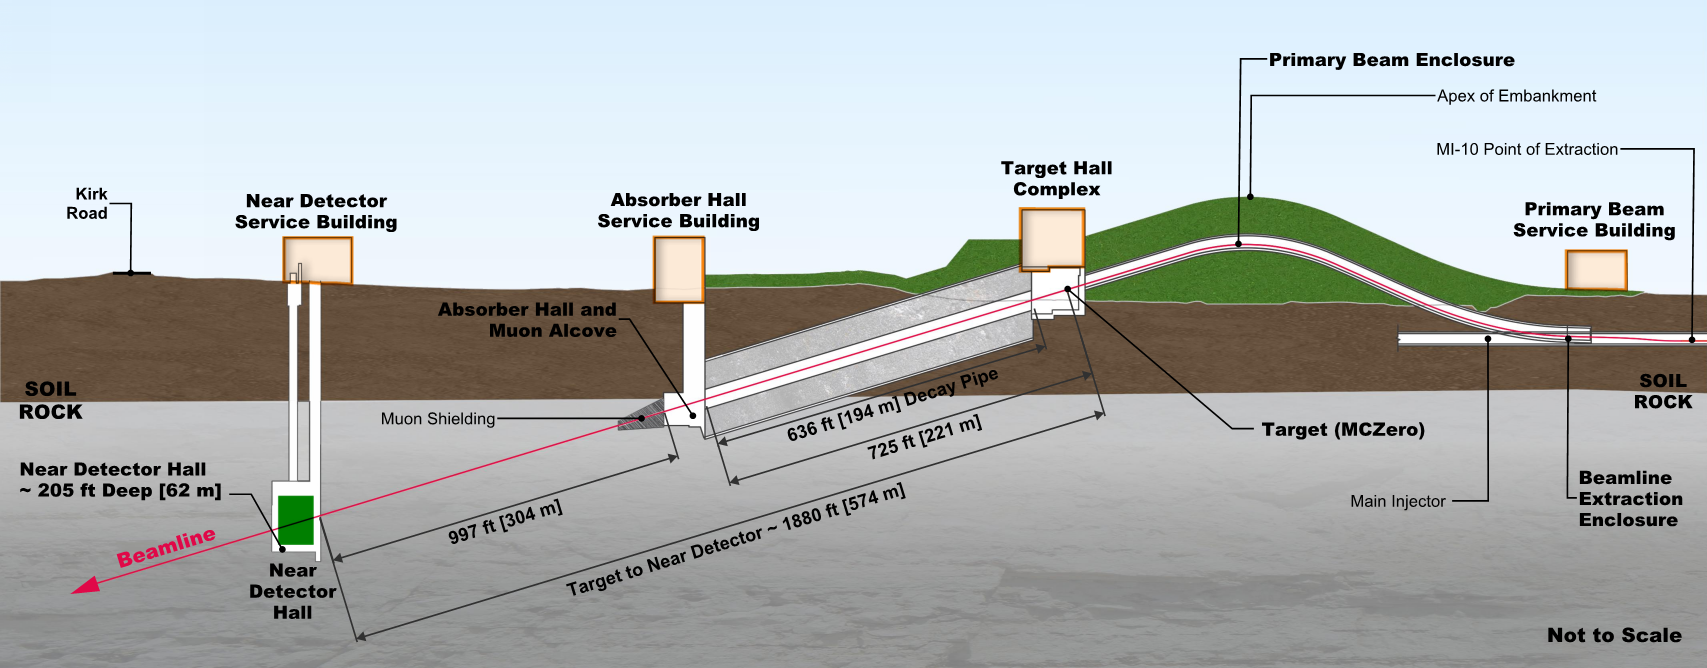
\includegraphics[width=0.95\linewidth]{Images/DUNE/LBNF/beamline-sideview}
	\caption[Schematic longitudinal section of the \gls{lbnf} beamline at Fermilab.]{Schematic longitudinal section of the \gls{lbnf} beamline at Fermilab (not to scale). Figure taken from Ref. \cite{DUNE2016CDR3}.}
	\label{fig:lbnf_beamline}
\end{figure}

\section{LBNF beamline}

The \gls{lbnf} project is responsible for producing the neutrino beam for the \gls{dune} detectors. A detailed discussion of the \gls{lbnf} programme can be found in the \gls{dune}/\gls{lbnf} \gls{cdr} Volume III \cite{DUNE2016CDR3}.

A schematic diagram of the longitudinal section of the \gls{lbnf} beamline is shown in Fig. \ref{fig:lbnf_beamline}. First, a beam of $60-120~\mathrm{GeV}$ protons is extracted from the Fermilab Main Injector. This beam is aimed towards the target area, where it collides with a cylindrical graphite target to produce charged pions and kaons.

The diffuse, secondary beam of particles is focused by a pair of magnetic horns. These select the positively charged particles when operated in Forward Horn Current (\gls{fhc}) mode, or the negatively charged ones when the current is reversed, also known as Reverse Horn Current (\gls{rhc}) mode. The focused secondary beam then enters a $194~\mathrm{m}$ decay pipe where the pions and kaons will predominantly produce $\mu^{+}\nu_{\mu}$ pairs when in \gls{fhc} mode (or $\mu^{-}\bar{\nu}_{\mu}$ in \gls{rhc} mode).

At the end of the decay pipe a hadron absorber removes the undecayed hadrons and muons from the beam, which reduces the $\nu_{e}$ ($\bar{\nu}_{e}$) and $\bar{\nu}_{\mu}$ ($\nu_{\mu}$) contamination  coming from the $\mu^{+}$ ($\mu^{-}$) decays. The resulting neutrino flux at the \gls{fd} is shown in Fig. \ref{fig:dune_fd_flux}, both for \gls{fhc} (left) and \gls{rhc} (right) modes. These predictions show the intrinsic $\overset{\brabarb}{\nu}_{e}$ contamination and wrong sign component from wrong sign and neutral meson decays, as well as muons decaying before reaching the absorber.

\begin{figure}[h!]
	\begin{subfigure}{0.49\textwidth}
		\centering
		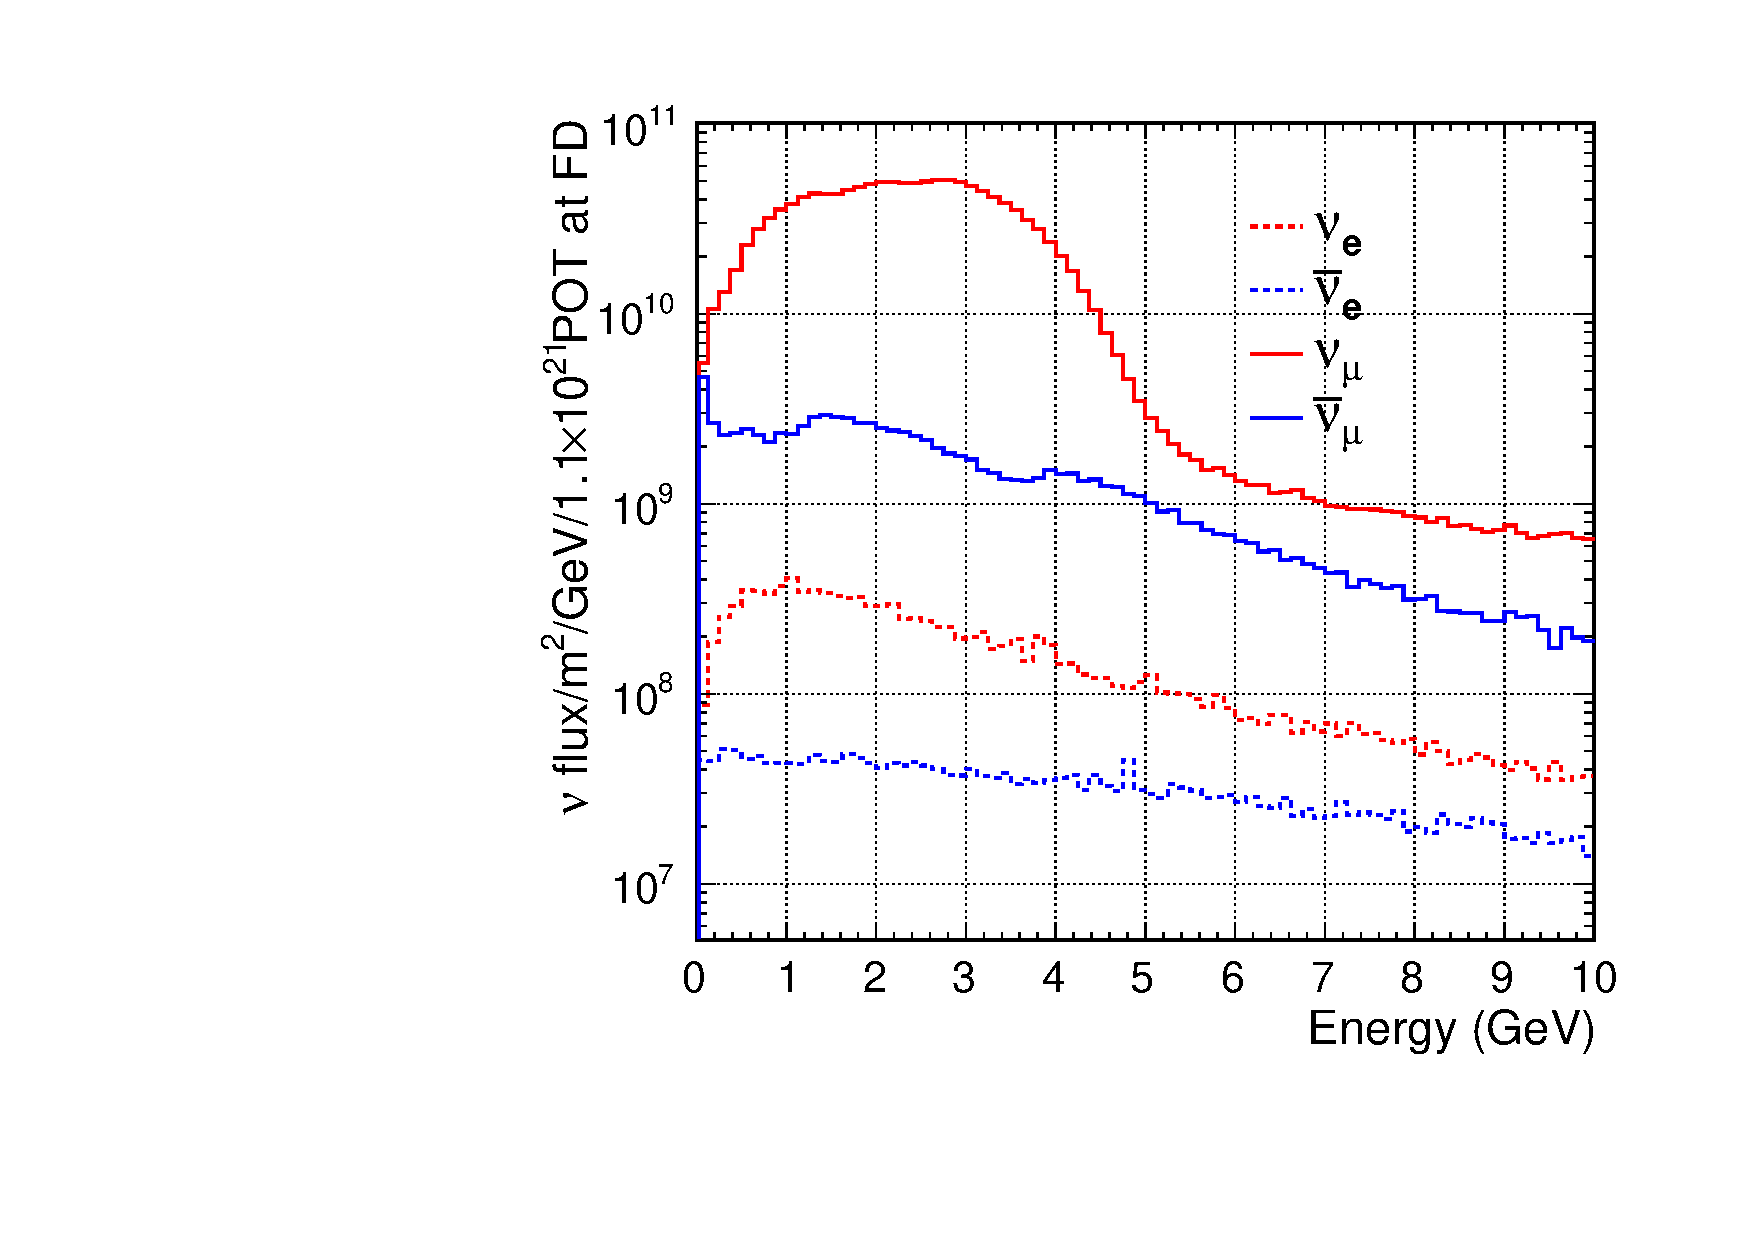
\includegraphics[width=.99\linewidth]{Images/DUNE/LBNF/dune_neutrino_fd_log}
	\end{subfigure}
	\begin{subfigure}{0.49\textwidth}
		\centering
		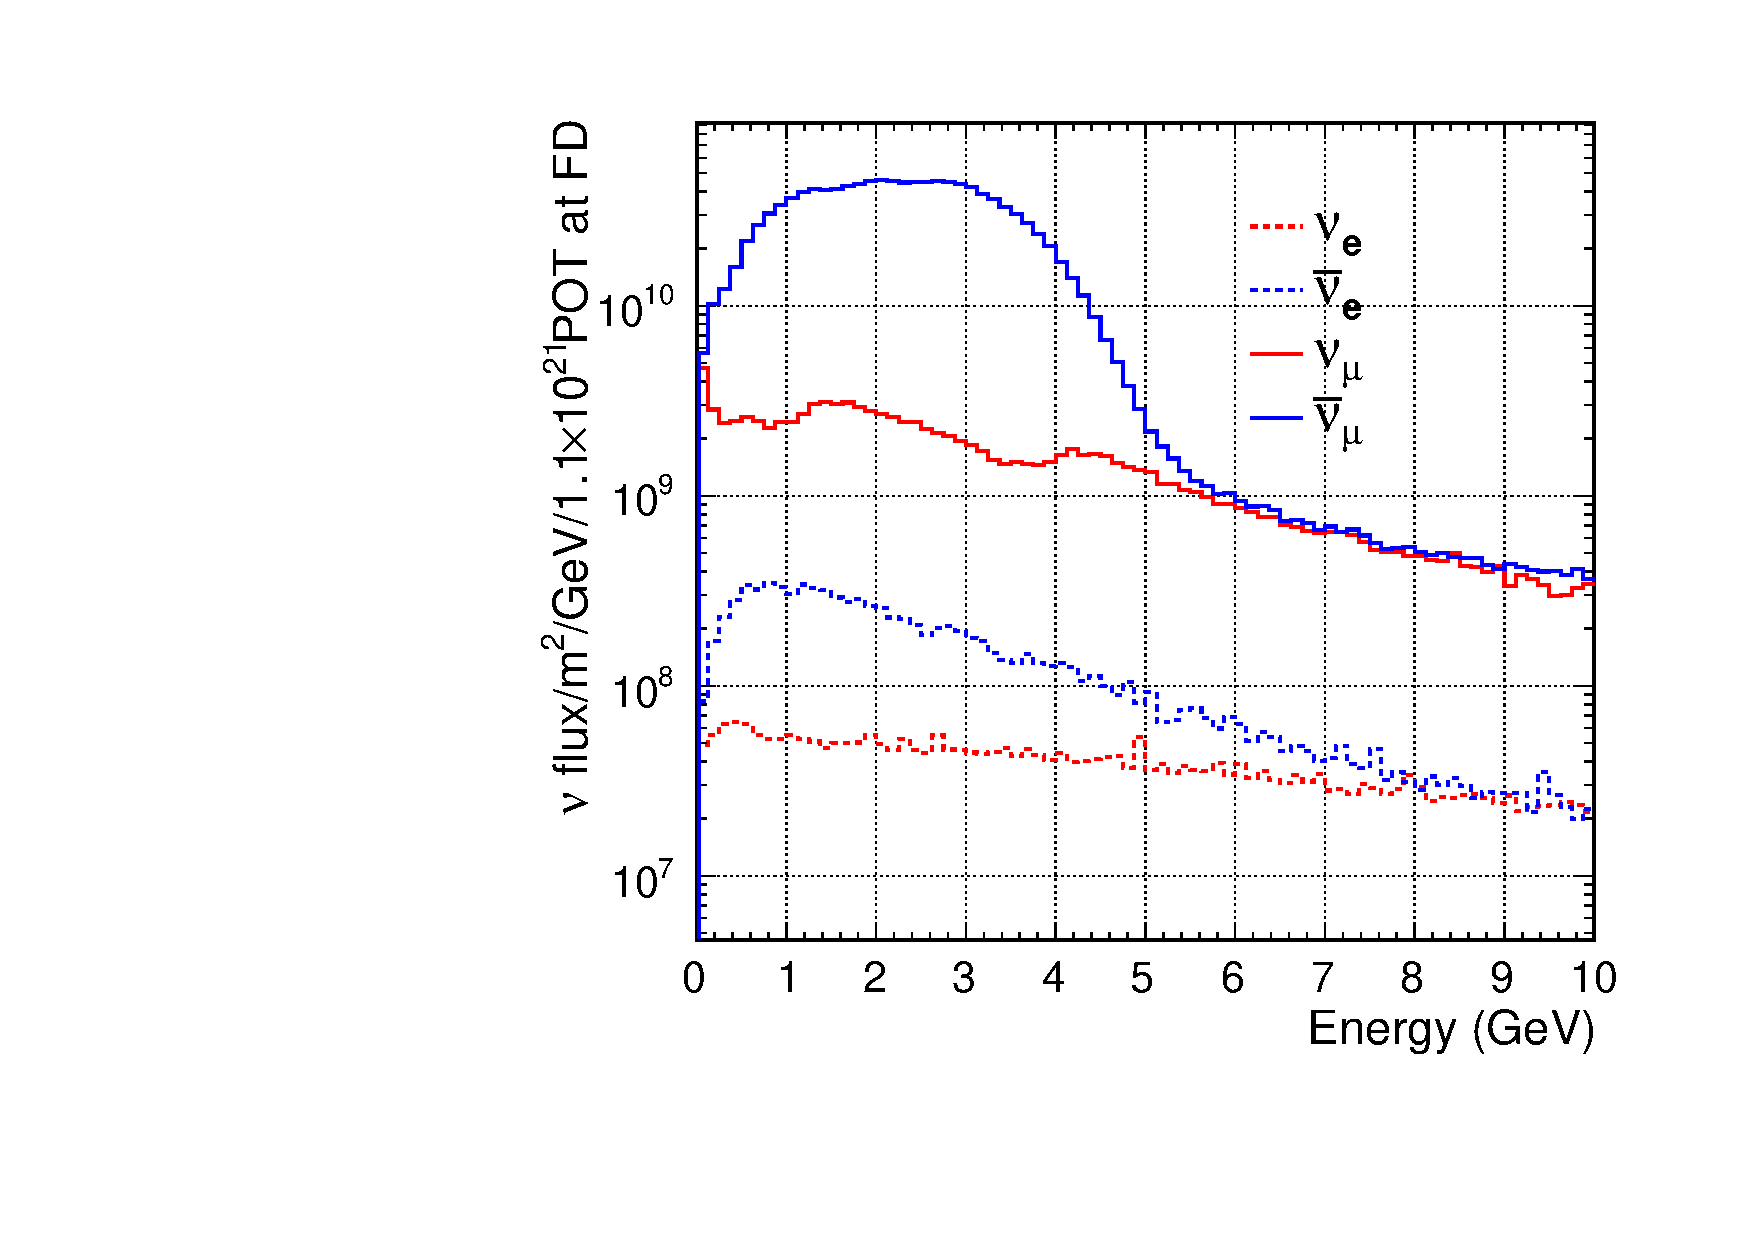
\includegraphics[width=.99\linewidth]{Images/DUNE/LBNF/dune_antineutrino_fd_log}
	\end{subfigure}
	\caption[Predicted neutrino fluxes at the \gls{fd} in \gls{fhc} mode and \gls{rhc} mode.]{Predicted neutrino fluxes at the \gls{fd} in \gls{fhc} mode (left panel) and \gls{rhc} mode (right panel). Figures taken from Ref. \cite{DUNE2020TDR2}.}
	\label{fig:dune_fd_flux}
\end{figure}

\section{Near Detector}

To estimate the oscillation parameters we measure the neutrino energy spectra at the \gls{fd}. This reconstructed energy arises from a convolution of the neutrino flux, cross section, detector response and the oscillation probability. Using theoretical and empirical models to account for the other effects, one can extract the oscillation probability using the measurement. However, these models have associated a number of uncertainties that are then propagated to the oscillation parameters.

\begin{figure}[t]
	\centering
	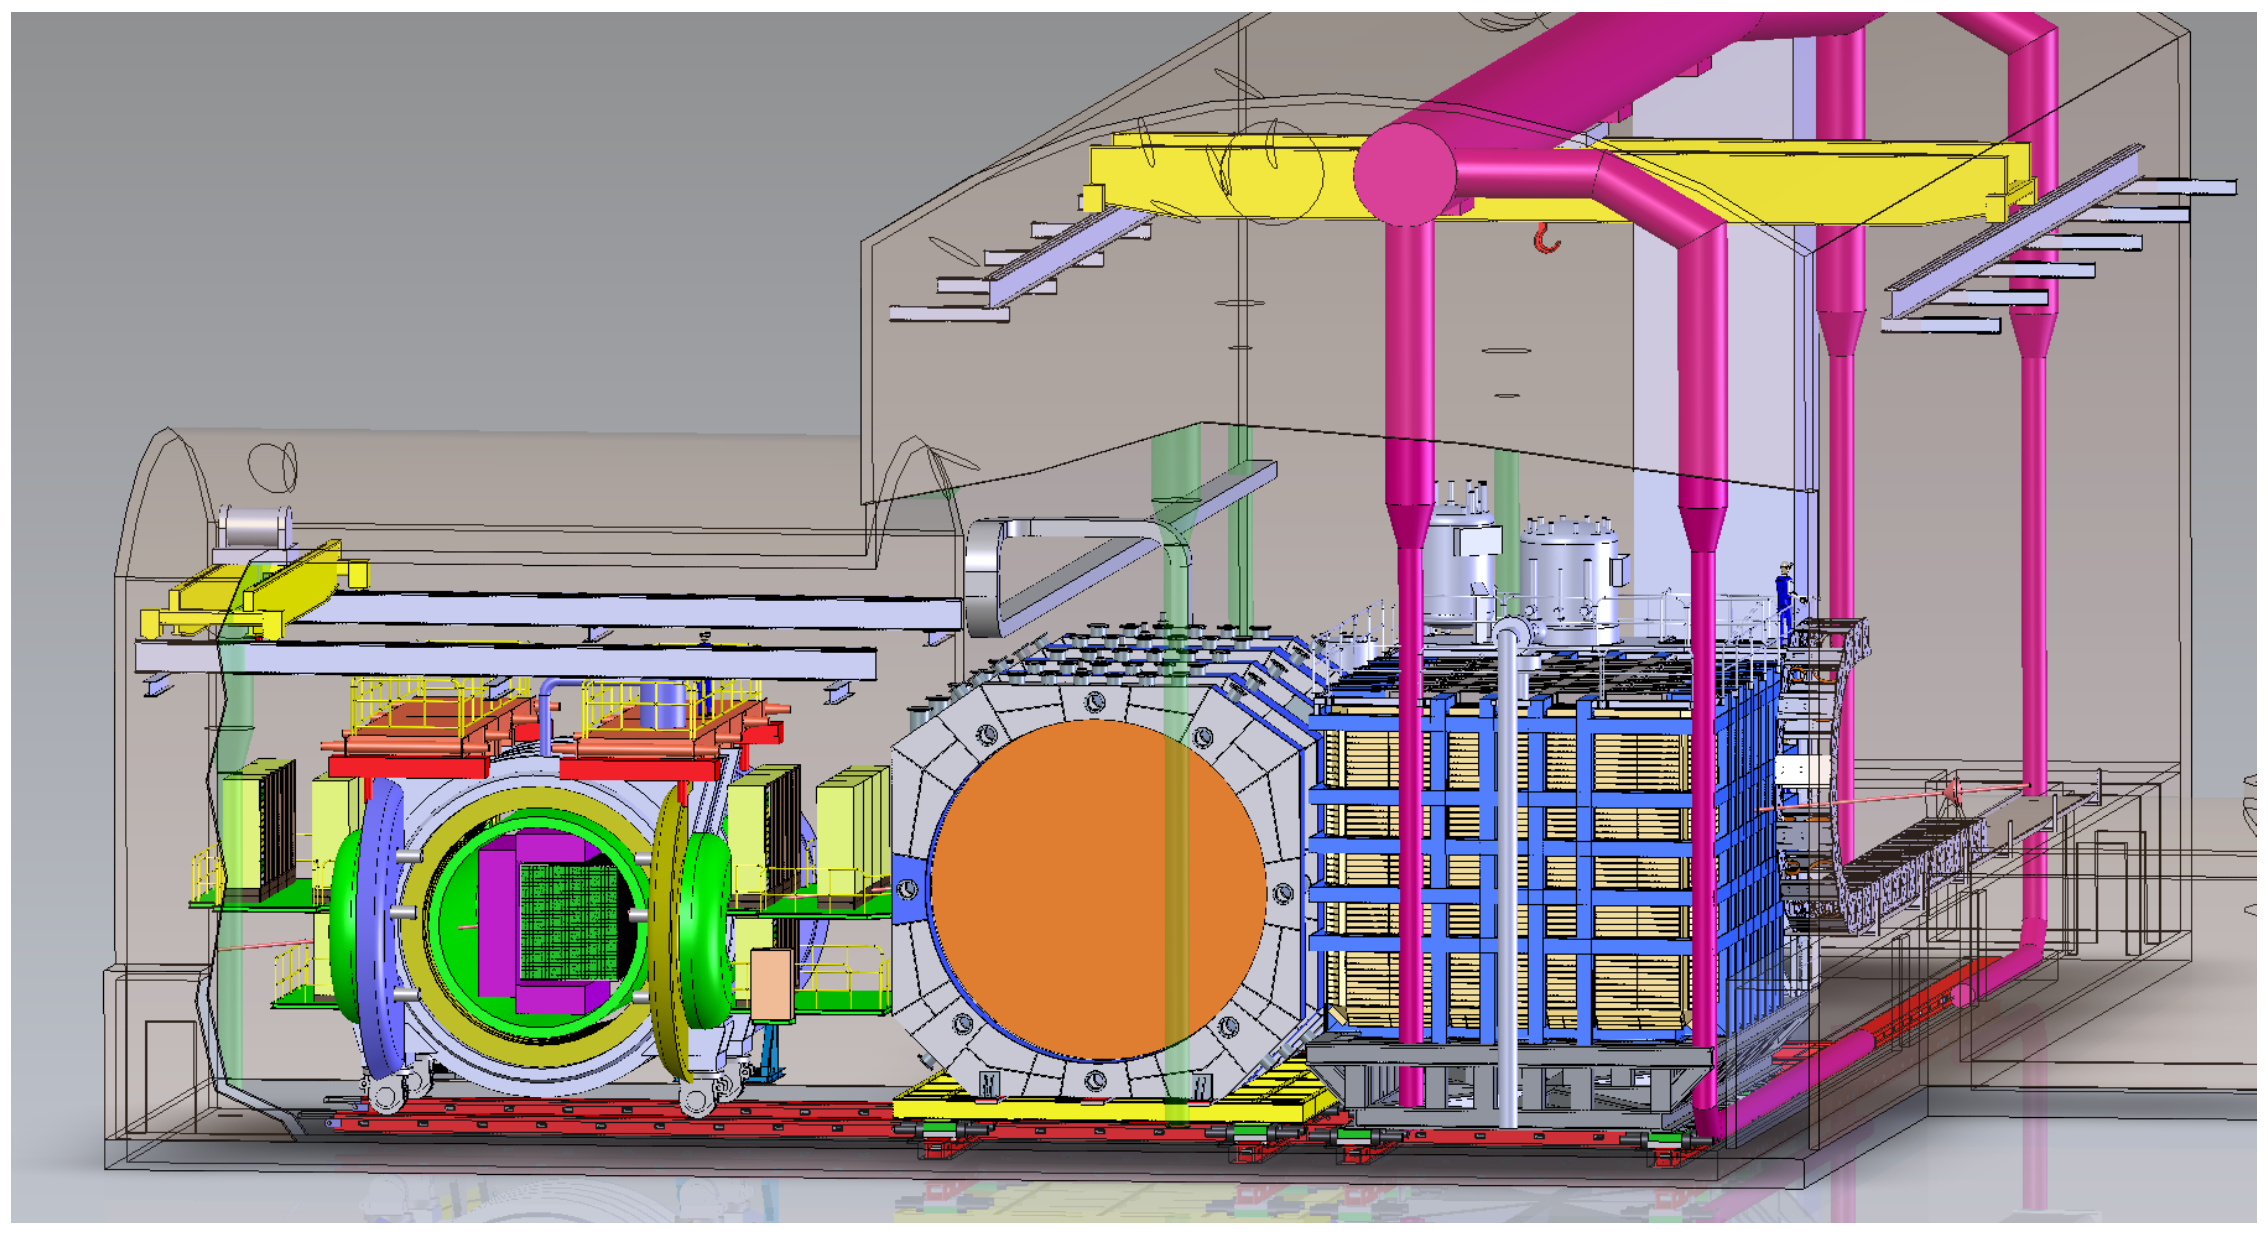
\includegraphics[width=0.95\linewidth]{Images/DUNE/ND/nd_hall}
	\caption[Representation of the \gls{nd} hall in Phase II.]{Representation of the \gls{nd} hall in Phase II, showing the different subcomponents. From right to left, in the direction of the beam, we have \gls{ndlar}, \gls{ndgar} and \gls{sand}. Figure taken from Ref. \cite{DUNE2021NDCDR}.}
	\label{fig:dune_nd}
\end{figure}

One of the main roles of the \gls{nd} is to measure the neutrino interaction rates before the oscillation effects become relevant, i.e. close to the production point. By measuring the $\nu_{\mu}$ and $\nu_{e}$ energy spectra, and that of their corresponding antineutrinos, at the \gls{nd} we can constrain the model uncertainties. A complete cancellation of the uncertainties when taking the ratio between the \gls{fd} and \gls{nd} measurements is not possible, as that would require both detectors to have identical designs and the neutrino fluxes seen by them to be the same. Because of the distance, the flux probed by the \gls{fd} will have a different energy and flavour composition than that at the \gls{nd}, as neutrinos oscillate and the beam spreads. The differences in the flux also determine the design of the detectors, therefore the \gls{nd} is limited in its capability to match the \gls{fd} design.

Nevertheless, having a highly capable \gls{nd}, \gls{dune} can minimise the systematic uncertainties affecting the observed neutrino energy. The \gls{nd} data can be used to tune the model parameters by comparison with the prediction. Then, one uses the tuned model to predict the unoscillated \gls{fd} spectra. Comparing the prediction with the measured spectra it is possible to extract the oscillation parameters.

\begin{comment}
	Another requirement for the \gls{nd} is that it must reduce the impact of the cross section uncertainties on the measurement of the neutrino spectra. In other words, it needs to measure neutrino interactions much more accurately than the \gls{fd}. This requires a better particle identification and energy reconstruction capabilities.
\end{comment}

\begin{figure}[t]
	\centering
	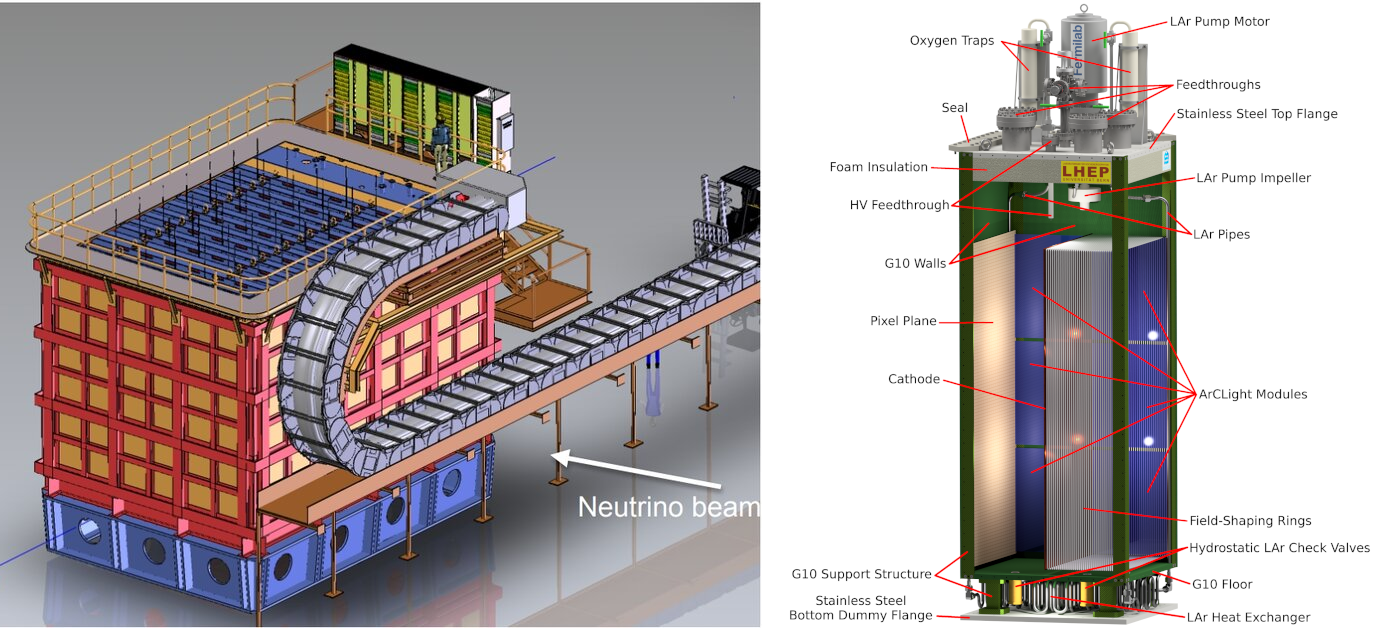
\includegraphics[width=0.99\linewidth]{Images/DUNE/ND/nd_lar_mod}
	\caption[Schematic representation of the external components of \gls{ndlar}, including the cryostat and the \gls{prism} movable system.]{Schematic representation of the external components of \gls{ndlar}, including the cryostat and the \gls{prism} movable system (left) and detailed drawing of one ArgonCube module (right). Figure adapted from Ref. \cite{DUNE2020TDR1}.}
	\label{fig:dune_nd_lar}
\end{figure}

Additionally, the \gls{nd} will have a physics programme of its own. In particular, it will measure neutrino cross sections that will then be used to constrain the model used in the long-baseline oscillation analysis. It will also be used to search for \gls{bsm} phenomena such as heavy neutral leptons, dark photons, millicharged particles, etc.

The \gls{dune} \gls{nd} can be divided in three main components, a \gls{lartpc} known as \gls{ndlar}, a magnetised muon spectrometer, which will be the Temporary Muon Spectrometer (\gls{tms}) in Phase I and \gls{ndgar} in Phase II, and the System for on-Axis Neutrino Detection (\gls{sand}). The layout of the Phase II \gls{dune} \gls{nd} can be seen in Fig. \ref{fig:dune_nd}. The first two components of the \gls{nd} will be able to move off-axis, in what is called the Precision Reaction-Independent Spectrum Measurement (\gls{prism}) concept. More details on the purpose and design of the \gls{nd} can be found in the \gls{dune} \gls{nd} Conceptual Design Report (\gls{cdr}) \cite{DUNE2021NDCDR}.

\subsection{ND-LAr}

\begin{figure}[t]
	\centering
	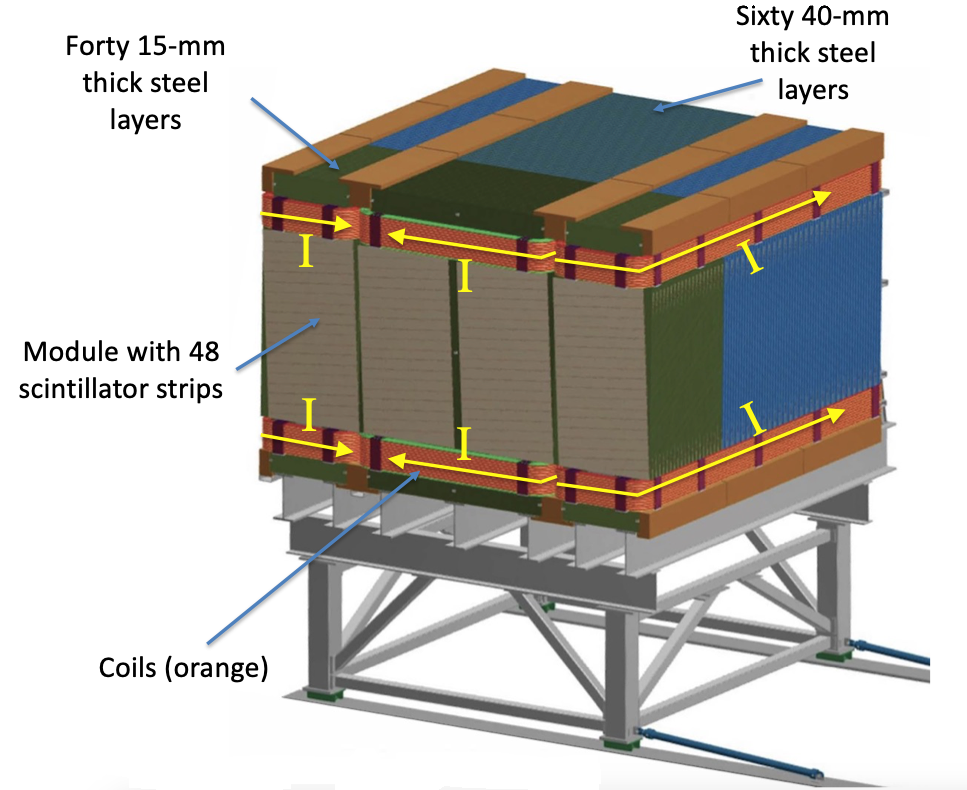
\includegraphics[width=0.65\linewidth]{Images/DUNE/ND/nd_tms}
	\caption[Schematic view of the \gls{tms} detector, highlighting its main parts.]{Schematic view of the \gls{tms} detector, highlighting its main parts. Figure adapted from Ref. \cite{Nehm2024}.}
	\label{fig:dune_tms}
\end{figure}

\gls{ndlar} is a \gls{lartpc}, as the \gls{nd} needs a \gls{lar} component to reduce cross section and detector systematic uncertainties in the oscillation analysis. However, its design differs significantly from those proposed for the \gls{fd} modules. Because of the high event rates at the \gls{nd}, approximately $55$ neutrino interaction events per $10~\mu\mathrm{s}$ spill, \gls{ndlar} will be built in a modular way. Each of the modules, based on the ArgonCube technology, is a fully instrumented, optically isolated \gls{tpc} with a pixelated readout \cite{Asaadi2019}. The pixelisation allows for full 3D reconstruction and the optical isolation reduces the problems due to overlapping interactions. Figure \ref{fig:dune_nd_lar} shows a representation of the external parts of \gls{ndlar} (left) and a detailed diagram of an ArgonCube module (right).

With a fiducial mass of $67~\mathrm{t}$ and dimensions $7~\mathrm{m} \ (\text{w}) \times 3~\mathrm{m} \ (\text{h}) \times 5~\mathrm{m} \ (\text{l})$, \gls{ndlar} will be able to manage high event rates and contain the hadronic systems from the beam neutrino interactions, but muons with a momentum higher than $0.7~\mathrm{GeV}/c$ will exit the detector.

\begin{figure}[t]
	\centering
	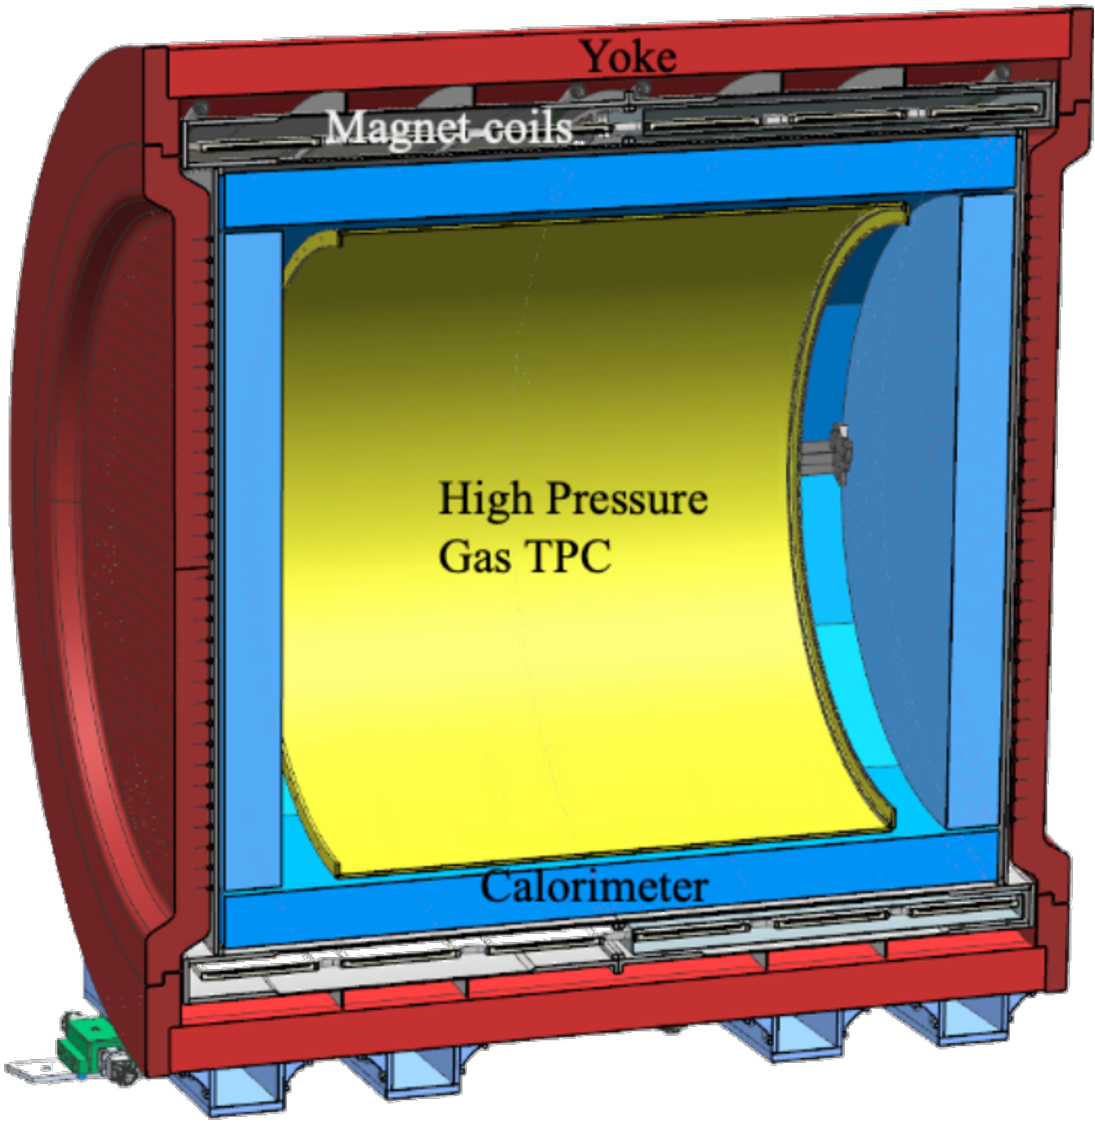
\includegraphics[width=0.45\linewidth]{Images/DUNE/ND/nd_gar}
	\caption[Cross section of the \gls{ndgar} geometry, showing the \gls{hpgtpc}, \gls{ecal} and magnet.]{Cross section of the \gls{ndgar} geometry, showing the \gls{hpgtpc}, \gls{ecal} and magnet. Figure adapted from Ref. \cite{DUNE2024Phase2}.}
	\label{fig:dune_nd_gar}
\end{figure}

\subsection{TMS/ND-GAr}

To accurately estimate the neutrino energy, the momentum of the outgoing muons needs to be determined. That is the reason why a muon spectrometer is needed downstream of \gls{ndlar}.

In Phase I that role will be fulfilled by \gls{tms}. It is a magnetised sampling calorimeter, with alternating steel and plastic scintillator layers. Figure \ref{fig:dune_tms} shows a schematic view of the \gls{tms} detector. The magnetic field allows a precise measurement of the sign of the muon, so one can distinguish between neutrino and antineutrino interactions.

After the Phase II upgrade, \gls{tms} will be replaced with a more capable near detector. The current technology considered is \gls{ndgar}. This detector is a magnetised, high-pressure gaseous argon (\gls{gar}) \gls{tpc} (often denoted as \gls{hpgtpc}) surrounded by an electromagnetic calorimeter (\gls{ecal}) and a muon tagger. A cross section of its geometry can be seen in Fig. \ref{fig:dune_nd_gar}. \gls{ndgar} will be able to measure the momenta of the outgoing muons while also detecting neutrino interactions inside the \gls{gar} volume. This allows \gls{ndgar} to constrain the systematic uncertainties even further, as it will be able to accurately measure neutrino interactions at low energies thanks to the lower tracking thresholds of the \gls{gar}.

\begin{figure}[t]
	\centering
	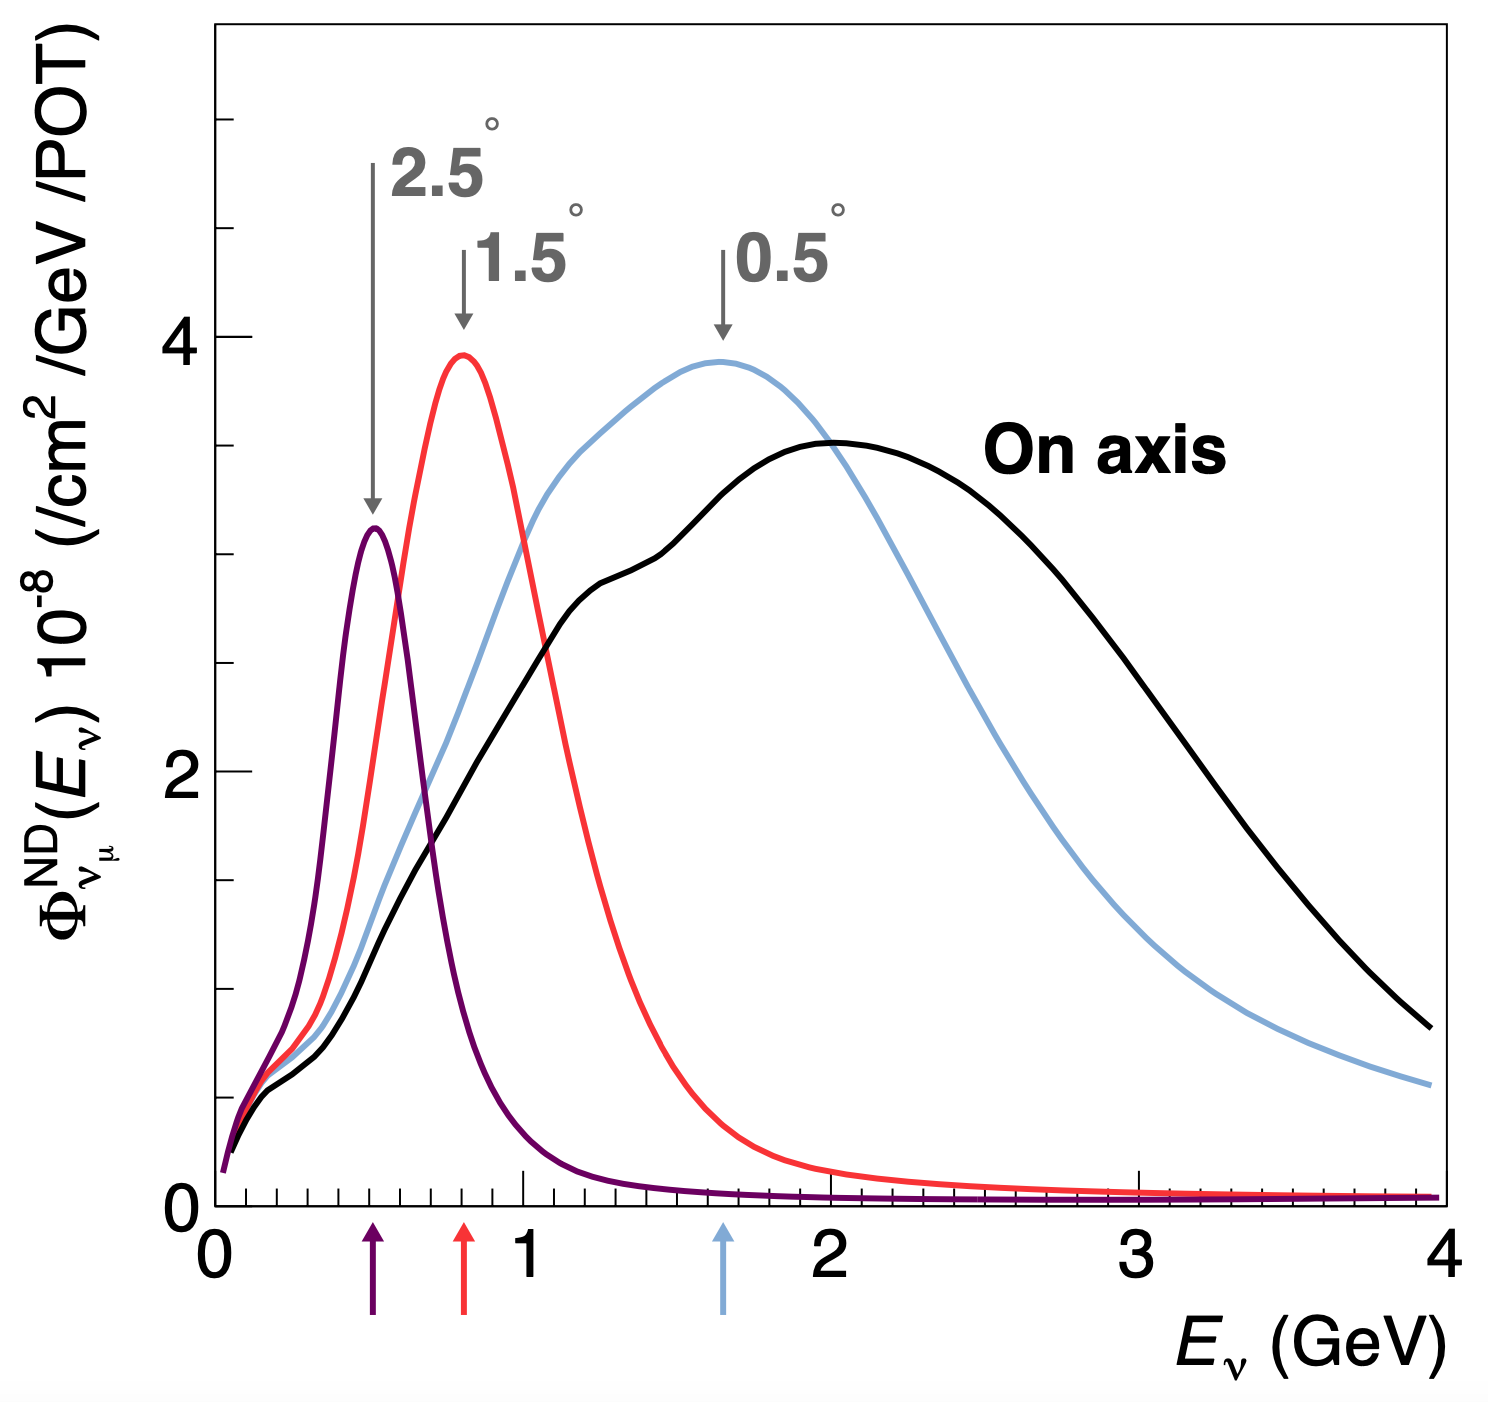
\includegraphics[width=0.55\linewidth]{Images/DUNE/ND/prism_spectra}
	\caption[Predicted beam muon neutrino flux at the \gls{nd} location for different off-axis positions.]{Predicted beam muon neutrino flux at the \gls{nd} location for different off-axis positions. Figure taken from Ref. \cite{DUNE2021NDCDR}.}
	\label{fig:dune_prism}
\end{figure}

\subsection{PRISM}

In general, the observed peak neutrino energy of a neutrino beam decreases as the observation angle with respect to the beam direction increases. This feature has been used in other long-baseline neutrino experiments, like \gls{t2k} ($2.5^{\circ}$ off-axis) and \gls{nova} ($0.8^{\circ}$ off-axis), to achieve narrower energy distributions. The \gls{dune} \gls{prism} concept exploits this effect using a movable \gls{nd}. Within \gls{prism} both \gls{ndlar} and the muon spectrometer (\gls{tms} in Phase I and \gls{ndgar} in Phase II) can be moved up to $3.2^{\circ}$ off-axis, equivalent to moving the detectors $30.5~\mathrm{m}$ laterally through the \gls{nd} hall.

This will allow us to record additional data samples with different energy compositions. Figure \ref{fig:dune_prism} compares the on-axis muon neutrino flux at the \gls{nd} with the fluxes at different off-axis positions. As the off-axis position increases the neutrino flux becomes closer to a monoenergetic beam with a lower peak energy. These samples can be used to perform a data-driven determination of the relation between true and reconstructed neutrino energy, to reduce the dependence on the interaction model. The off-axis samples are linearly combined to produce a narrow Gaussian energy distribution centered on the target true energy. From the combination coefficients one can build a sample of reconstructed neutrino events that will determine the energy mapping.

The \gls{prism} samples will also be used to form a flux at the \gls{nd} location similar in shape to the oscillated flux measured by the \gls{fd}. This method can be used to extract the oscillation parameters with minimal input from the neutrino interaction model \cite{Hasnip2023}.

\subsection{SAND}

The role of \gls{sand} is to monitor the beam stability by measuring the on-axis neutrino energy spectra. As the \gls{prism} programme requires that \gls{ndlar} and its downstream muon spectrometer spend about half of the time in off-axis positions, it is not possible to monitor the stability of the beam with the movable detectors. Moreover, for the success of \gls{prism} it is essential to have a stable beam configuration, or at least a quick assessment and modeling of the distortions.

The \gls{sand} detector is magnetised, and features an inner low density tracker, a \gls{lar} target with optical readout and a surrounding sampling calorimeter.

\section{A More Capable Near Detector}\label{sec:mcnd}

In \gls{dune} Phase II, a more capable near detector is needed to achieve the ultimate physics goals of the experiment. The current leading proposal for this detector is \gls{ndgar}. As mentioned previously, it will fulfill the role of \gls{tms}, measuring the momentum and sign of the charged particles exiting \gls{ndlar}. Additionally, it will be able to measure neutrino interactions inside the \gls{hpgtpc}, achieving lower energy thresholds than those of the \gls{nd} and \gls{fd} \gls{lartpc}s. It will also provide a uniform event acceptance, similar to the \gls{fd}, which could not be achieved by \gls{ndlar} + \gls{tms}. By doing so, \gls{ndgar} will allow to constrain the relevant systematic uncertainties for the \gls{lbl} analysis even further. A detailed discussion on the requirements, design, performance and physics of \gls{ndgar} can be found in the \gls{dune} \gls{nd} \gls{cdr} \cite{DUNE2021NDCDR} and the \gls{ndgar} white paper \cite{DUNE2022GArWhite}.

\subsection{Requirements}

The primary requirement for \gls{ndgar} is to measure the momentum and charge of muons from $\nu_{\mu}$ and $\bar{\nu}_{\mu}$ \gls{cc} interactions in \gls{ndlar}, in order to measure their energy spectrum. To achieve the sensitivity to the neutrino oscillation parameters described in the \gls{dune} \gls{fd} \gls{tdr} Volume II \cite{DUNE2020TDR2}, \gls{ndgar} should be able to constrain the muon energy within a $1\%$ uncertainty or better.

Another requirement for \gls{ndgar} is the precise measurement of neutrino interactions on argon for the energies relevant to the neutrino oscillation program. The goal is to constrain the cross section systematic uncertainties in the regions of phase space that are not accessible to \gls{ndlar}. This requires the kinematic acceptance for muons in \gls{ndgar} to exceed that of \gls{ndlar}, being comparable to that observed in the \gls{fd}.

\gls{ndgar} should also be able to help establish the relationship between true and reconstructed energy from neutrino interactions on argon, being sensitive to particles that are not observed or may be misidentified in \gls{ndlar}. In particular, \gls{ndgar} needs to have low tracking thresholds in order to measure the spectrum of pions and protons produced in final-state interactions (\gls{fsi}). It also must be able to accurately measure the pion multiplicity in 1, 2 and 3 pion final states, to inform the pion mass correction in the \gls{lartpc}s.

\subsection{Reference design}\label{subsec:ndgar_design}

The final design of \gls{ndgar} is still under preparation. However, a preliminary baseline design was in place at the time of the \gls{nd} \gls{cdr}. This section summarises the main features of that design, as it is also the one used by default in our simulation. The different options under consideration for the \gls{ndgar} design are further discussed in the \gls{dune} Phase II white paper \cite{DUNE2024Phase2}.

\subsubsection{HPgTPC}

The reference design for the \gls{ndgar} \gls{hpgtpc} follows closely that of the \gls{alice} \gls{tpc} \cite{ALICE2006}. It is a cylinder with a central high-voltage cathode, generating the electric field for the two drift volumes, with a maximum drift distance of $2.5~\mathrm{m}$ each. The anodes will be instrumented with charge readout chambers. The original design repurposed the multi-wire proportional readout chambers (\gls{mwpc}s) of \gls{alice}. However, some of the current R\&D efforts focus on a gas electron multiplier (\gls{gem}) \cite{Sauli1997} option instead. Figure \ref{fig:alice_tpc} shows a schematic diagram of the \gls{alice} \gls{tpc} design. The basic \gls{ndgar} geometry will resemble this, except for the inner field cage.

\begin{figure}[t]
	\centering
	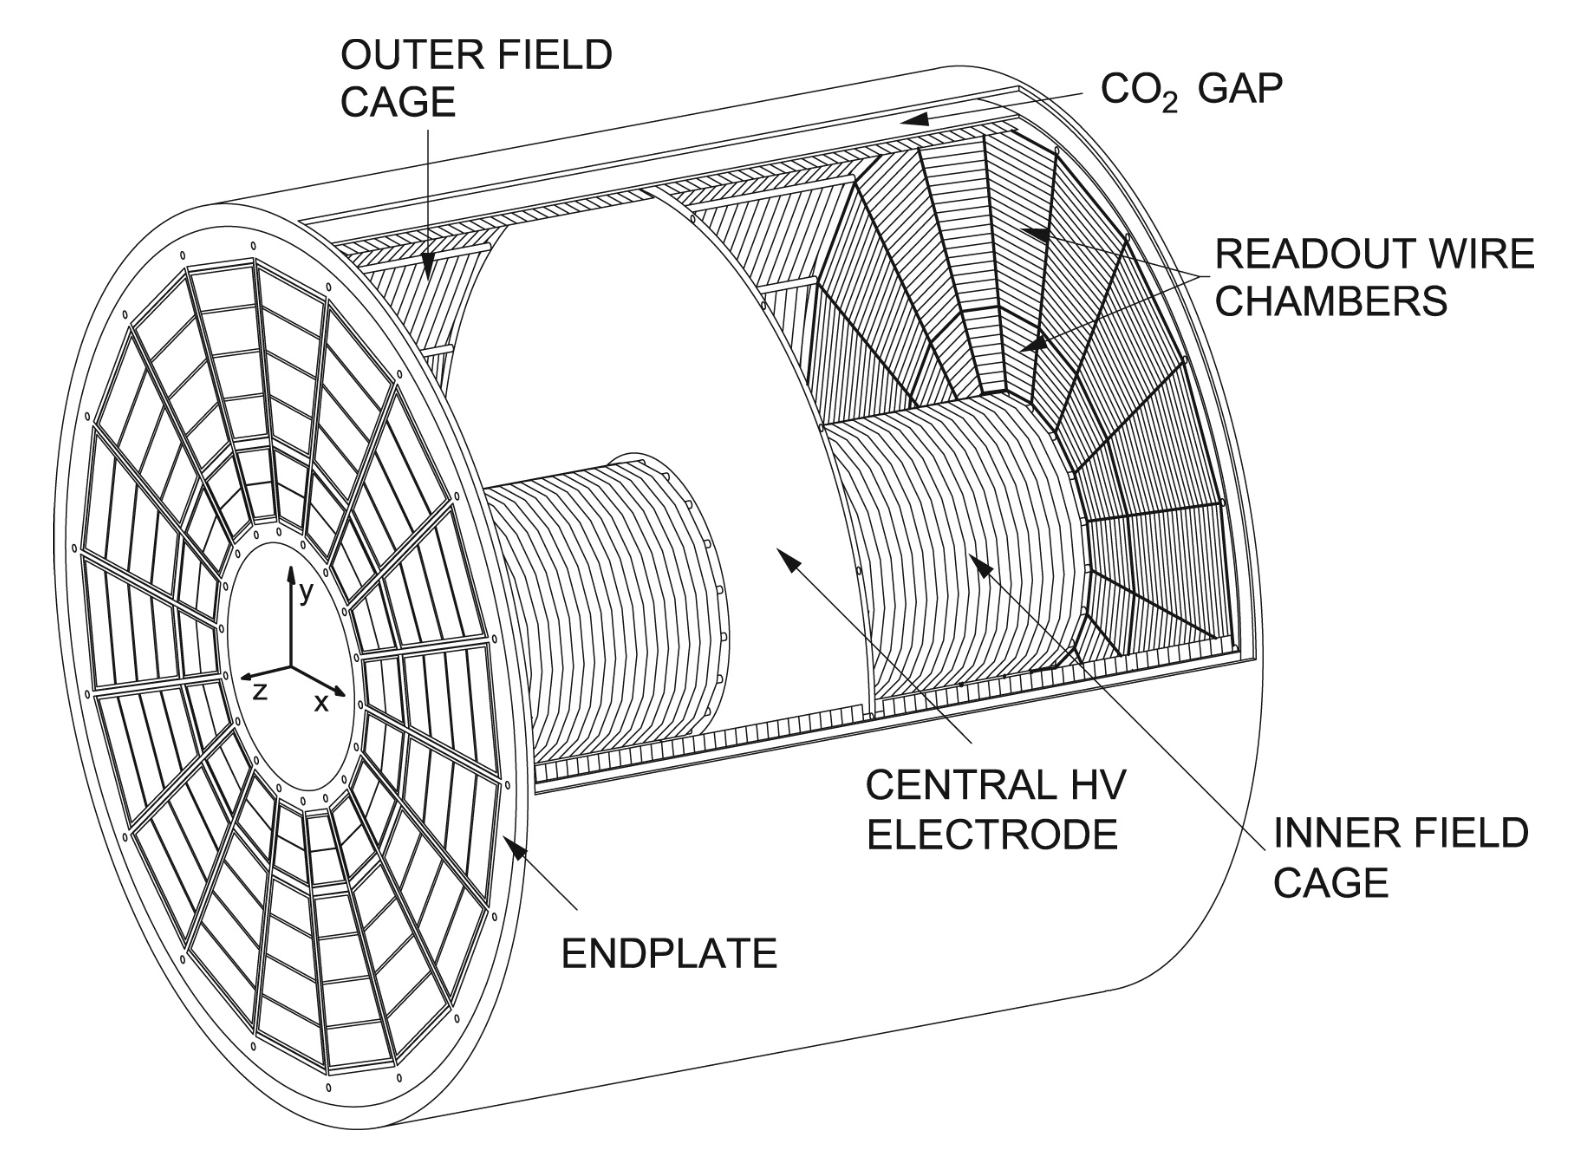
\includegraphics[width=0.7\linewidth]{Images/ND-GAr/alice_tpc}
	\caption[Diagram of the \gls{alice} \gls{tpc}, showing the two drift chambers, inner and outer field cages and readout chambers.]{Diagram of the \gls{alice} \gls{tpc}, showing the two drift chambers, inner and outer field cages and readout chambers. Figure taken from Ref. \cite{DUNE2021NDCDR}.}
	\label{fig:alice_tpc}
\end{figure}

\gls{ndgar} will use a 90:10 molar fraction $\mathrm{Ar}$:$\mathrm{CH}_{4}$ mixture at $10~\mathrm{bar}$. With this baseline gas mixture light collection is not possible, as the quenching gas absorbs most of the \gls{vuv} photons. Additional R\&D efforts are underway, to understand if different mixtures allow for the light signal to be used to provide a $t_{0}$ while maintaining stable charge gain.

\subsubsection{ECal}

\begin{figure}[t]
	\centering
	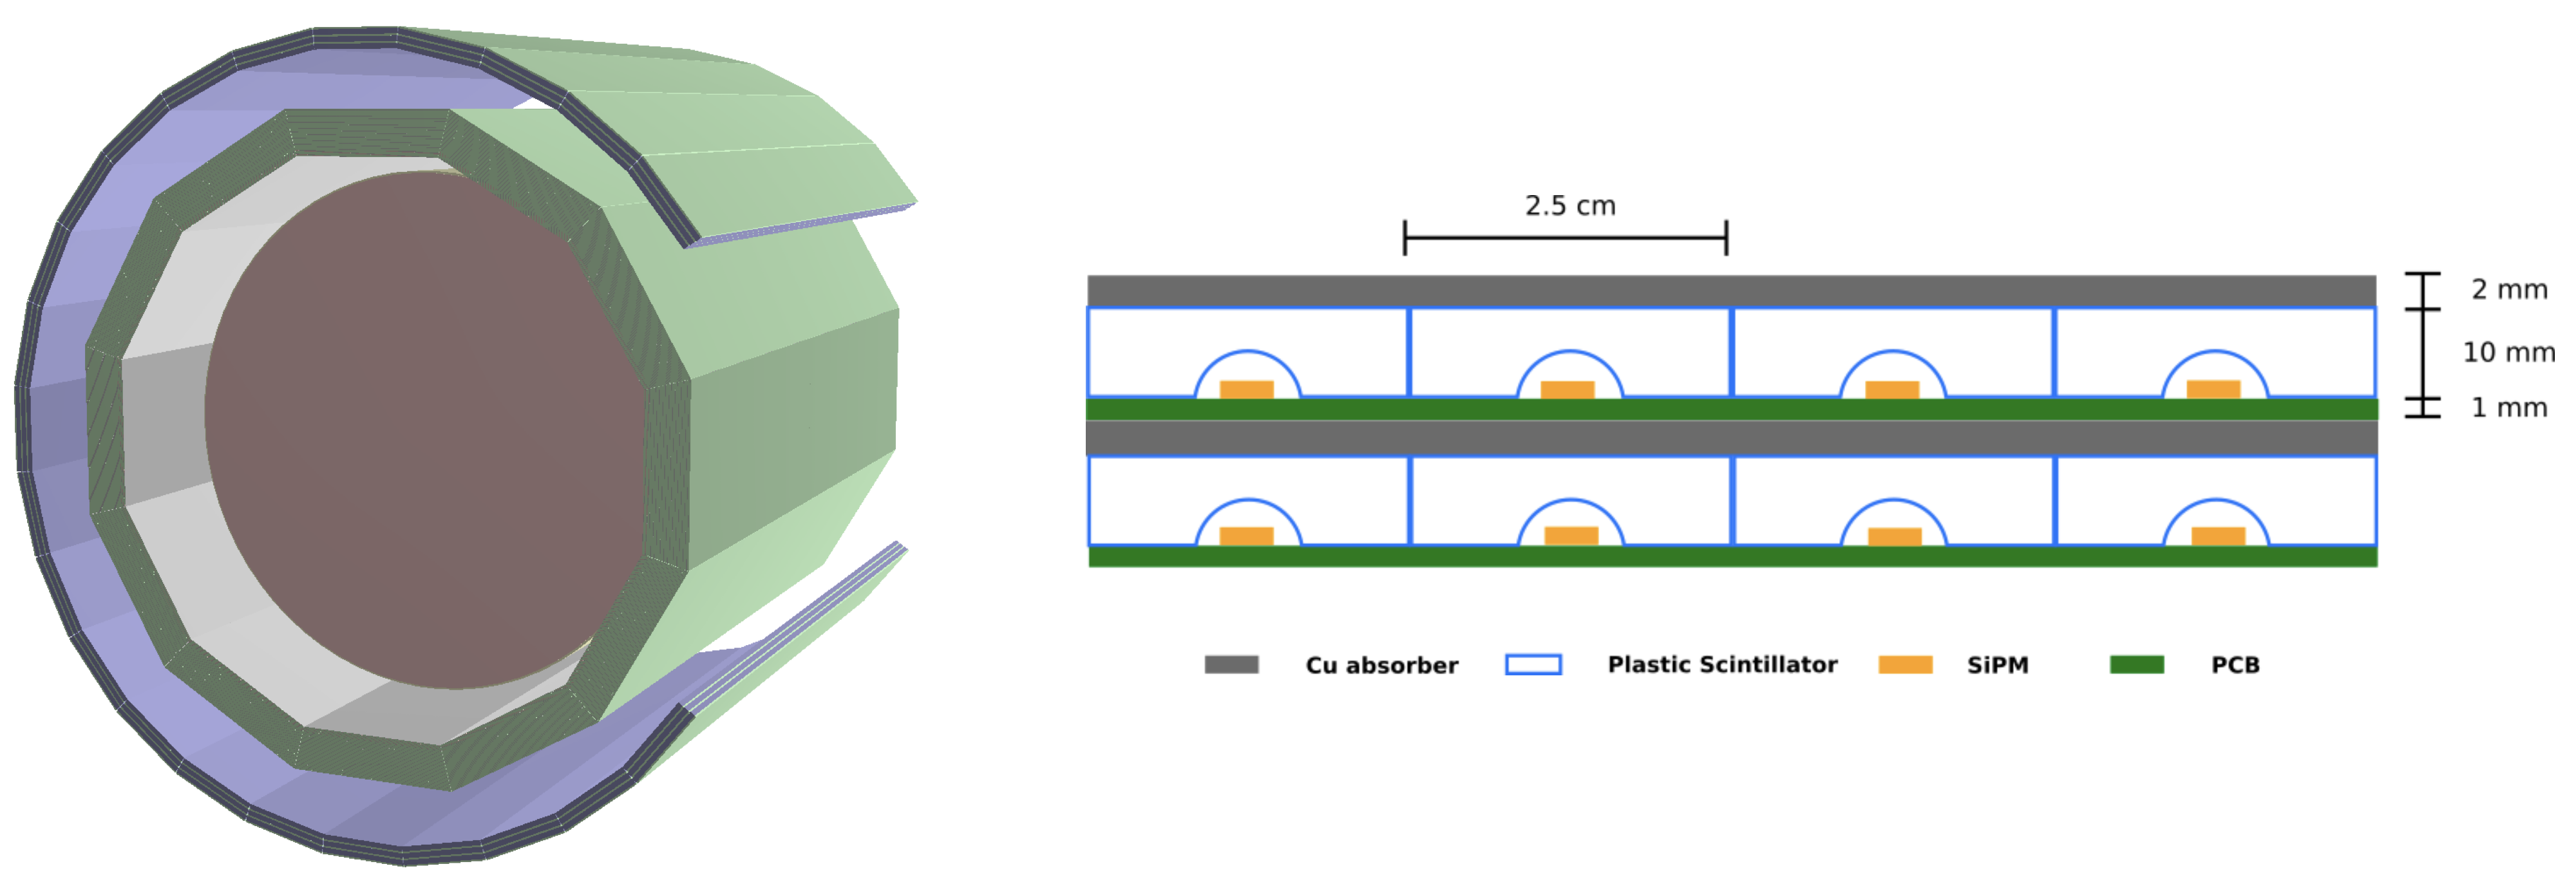
\includegraphics[width=0.99\linewidth]{Images/ND-GAr/ndgar_ecal}
	\caption[View of the 12-sided \gls{ecal} barrel and outer muon tagger geometries of \gls{ndgar}.]{View of the 12-sided \gls{ecal} barrel and outer muon tagger geometries (left) and layout of the \gls{ecal} tile layers for the $5~\mathrm{mm}$ Pb, $7~\mathrm{mm}$ scintillator option (right). Figure adapted from Ref. \cite{DUNE2021NDCDR}.}
	\label{fig:ndgar_ecal}
\end{figure}

The main role of the \gls{ndgar} \gls{ecal} is the calorimetric measurement of the electron energies and the reconstruction of photons, in particular those from neutral pion decays. Also, the \gls{ecal} is able to provide a $t_{0}$ timestamp for neutrino interactions, by associating its activity to the tracks in the \gls{hpgtpc}. The \gls{ecal} will also be able to perform neutron reconstruction using time-of-flight measurements, and reject external backgrounds thanks to its sub-nanosecond time resolution.

The \gls{ecal} design features three independent subdetectors, two end caps at each side and a barrel surrounding the \gls{hpgtpc}. Each of the detectors is divided in modules, which combine alternating layers of plastic scintillator and absorber material read out by silicon photomultipliers (\gls{sipm}s). The inner scintillator layers consist of $2.5\times2.5~\mathrm{cm}^{2}$ high-granularity tiles, whereas the outer layers are made out of $4~\mathrm{cm}$ wide cross-strips spanning the whole module length. The current barrel geometry consists of 8 tile layers and 34 strip layers, while the end caps feature 6 and 36 respectively. The scintillator (Pb absorber) layers are $7~\mathrm{mm}$ ($5~\mathrm{mm}$) thick. The 12-sided geometry of the \gls{ecal} barrel (left) and the layout of the tile layers (left) can be seen in Fig. \ref{fig:ndgar_ecal}. This design was inspired by the \gls{calice} analog hadron calorimeter prototype \cite{CALICE2010}.

\subsubsection{Magnet}

The \gls{ndgar} magnet design, known as the Solenoid with Partial Yoke (\gls{spy}), consists of two coupled solenoids with an iron return yoke \cite{DUNESPY2023}. The idea behind the design is to have a solenoid as thin as possible, as well as a return yoke mass distribution that minimises the material budget between \gls{ndlar} and \gls{ndgar}. The magnet needs to provide a $0.5~\mathrm{T}$ field in the direction perpendicular to the beam, parallel to the drift electric field. It needs to host the pressure vessel and the surrounding \gls{ecal}, which points to an inner diameter of $\sim6.4~\mathrm{m}$.

The solenoid is a single layer coil, based on niobium titanium superconducting Rutherford cable. The total length of the coil is $7.5~\mathrm{m}$. The bobbin will be split in four segments, grouped in pairs with two identical cryostats connected in series. The iron yoke features an aperture in the upstream side, to minimise the energy loss of the muons coming from \gls{ndlar}. Still, its material will be enough to reduce the magnetic field reaching \gls{sand}, and also stop the charged pions produced inside the \gls{hpgtpc}.

\subsubsection{Muon system}

The design of the \gls{ndgar} muon system is still in a preliminary stage. Its role is to distinguish between muons and pions punching through the \gls{ecal}. This is especially important for wrong-sign determination, to separate the background $\bar{\nu}_{\mu}$ \gls{cc} interactions from neutral current events.

In its current form, the muon system consists of three layers of longitudinal sampling structures. It alternates $10~\mathrm{cm}$ Fe absorber slabs with $2~\mathrm{cm}$ plastic scintillator strips. The transverse granularity required is still under study.

\subsection{R\&D efforts}

\begin{figure}[t]
	\centering
	\includegraphics[width=0.99\linewidth]{Images/ND-GAr/toad.png}
	\caption[Photographs of the \gls{toad} pressure vessel at RHUL.]{Photographs of the \gls{toad} pressure vessel at RHUL. The \gls{tpc} is mounted inside the vessel, and the \gls{oroc} is supported by an aluminium frame. Figure taken from Ref. \cite{Ritchie-Yates2023}.}
	\label{fig:toad}
\end{figure}

There are several \gls{ndgar}-related prototypes, mostly focused on the \gls{tpc} charge readout and electronics. The priority is to test the full readout chain, in a high-pressure environment, using a gas mixture with high argon fraction. A detailed summary of these can be found in the \gls{dune} Phase II white paper \cite{DUNE2024Phase2}.

\subsubsection{Multi-Wire Proportional Chambers}

As mentioned before, the original \gls{ndgar} design repurposes the \gls{mwpc}s of the \gls{alice} \gls{tpc}, which became available after the recent upgrade \cite{ALICETPC2020}. These were operated using a 90:10:5 $\mathrm{Ne}$:$\mathrm{CO}_{2}$:$\mathrm{N}_{2}$ gas mixture at $1~\mathrm{atm}$. Therefore, their performance needed to be studied in an argon gas environment at high pressure.

The Gas-argon Operation of \gls{alice} \gls{tpc} (\gls{goat}) test stand tested the \gls{alice} readout chambers at high pressure. In particular, it used one of the previously operated \gls{alice} inner \gls{mwpc}s, also known as inner readout chambers (\gls{iroc}), in a pressure vessel rated to $10~\mathrm{atm}$. It measured the gas gain at various pressure points, voltages and gas mixtures.

The Test stand of an Overpressure Argon Detector (\gls{toad}) tested an \gls{alice} outer \gls{mwpc}, also known as outer readout chamber (\gls{oroc}), up to $5~\mathrm{atm}$. During its time at RHUL, it was used to study the achievable gas gain of the \gls{oroc} \cite{Ritchie-Yates2023}. At the moment, it is being commissioned at Fermilab for a full detector test of the readout electronics and the \gls{daq}.

Figure \ref{fig:toad} shows the interior of the \gls{toad} pressure vessel. The \gls{tpc} is mounted inside the vessel on three rails. The back of the \gls{oroc}, supported by an aluminium frame, can be seen at the front.

\begin{figure}[t]
	\begin{subfigure}{0.49\textwidth}
		\centering
		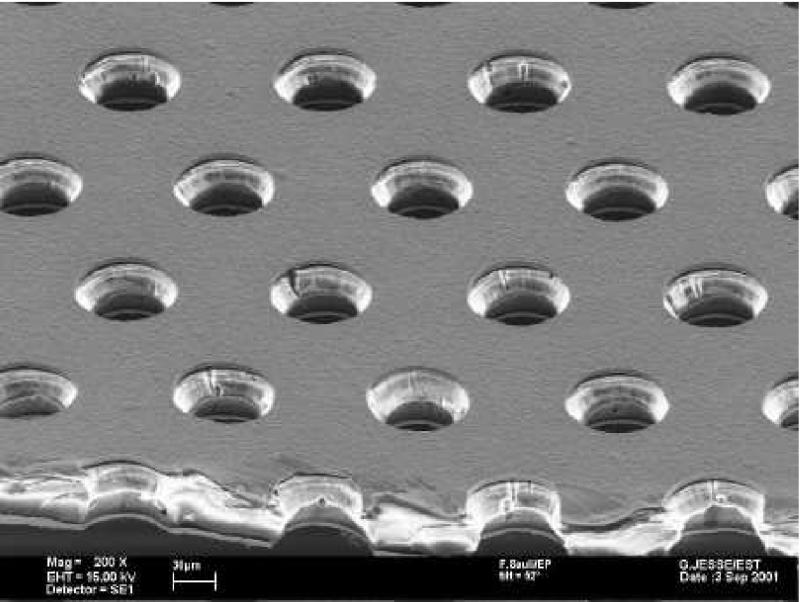
\includegraphics[width=.90\linewidth]{Images/ND-GAr/GEM_photo.jpg}
	\end{subfigure}
	\begin{subfigure}{0.49\textwidth}
		\centering
		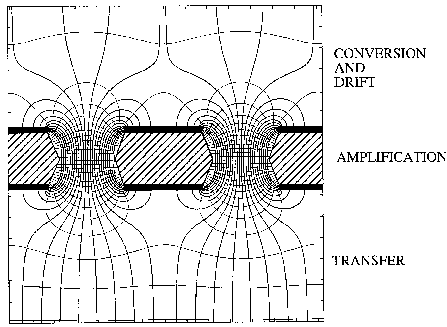
\includegraphics[width=.90\linewidth]{Images//ND-GAr/GEM_diagram.pdf}
	\end{subfigure}
	\caption[Electron microscope image and schematic diagram of a \gls{gem} electrode.]{Left panel: electron microscope image of a $50~\mu\mathrm{m}$ thick \gls{gem} electrode, with hole pitch and diameter of $140$ and $70~\mu\mathrm{m}$, respectively. Right panel: Schematics of a \gls{gem} electrode cross section, showing the electric field lines around the holes. Figures taken from Ref. \cite{Sauli2016}.}
	\label{fig:gem}
\end{figure}

\subsubsection{Gas Electron Multiplier}

An alternative to the \gls{mwpc} option is the use of \gls{gem}s. These are a type of micro-pattern detector, where the ionisation electrons passing through the holes in the \gls{gem} layers are accelerated by a high-intensity electric field. The acceleration causes the electrons to ionise the medium, resulting in an avalanche which increases the signal exponentially \cite{Sauli1997}. \gls{gem}s are used in numerous experiments that need a high spatial resolution, like \gls{alice} \cite{Lippmann2016} and \gls{cms} \cite{Calabria2016} after their upgrades.

Figure \ref{fig:gem} (left panel) shows an electron microscope picture of a $50~\mu\mathrm{m}$ thick \gls{gem} electrode, with a pitch between neighbouring holes of $140~\mu\mathrm{m}$ and a hole diameter of $70~\mu\mathrm{m}$. A schematic representation of the cross section of a \gls{gem} layer is shown in Fig. \ref{fig:gem} (left panel).

The Gaseous Argon T0 (\gls{gato}\footnote{Spanish for cat.}) prototype studies the use of thick \gls{gem}s made out of glass to achieve optical imaging of the primary ionisation. Using a $10~\mathrm{atm}$ pressure vessel, the goal is to study different argon-based mixtures that allow for a precise $t_{0}$ determination.

The \gls{gem} Over-pressurized with Reference Gases (\gls{gorg}\footnote{Persian for wolf.}) test stand is currently testing a \gls{gem}-based charge readout, using a triple-\gls{gem} stack.

\section{Far Detector}

\begin{figure}[t]
	\centering
	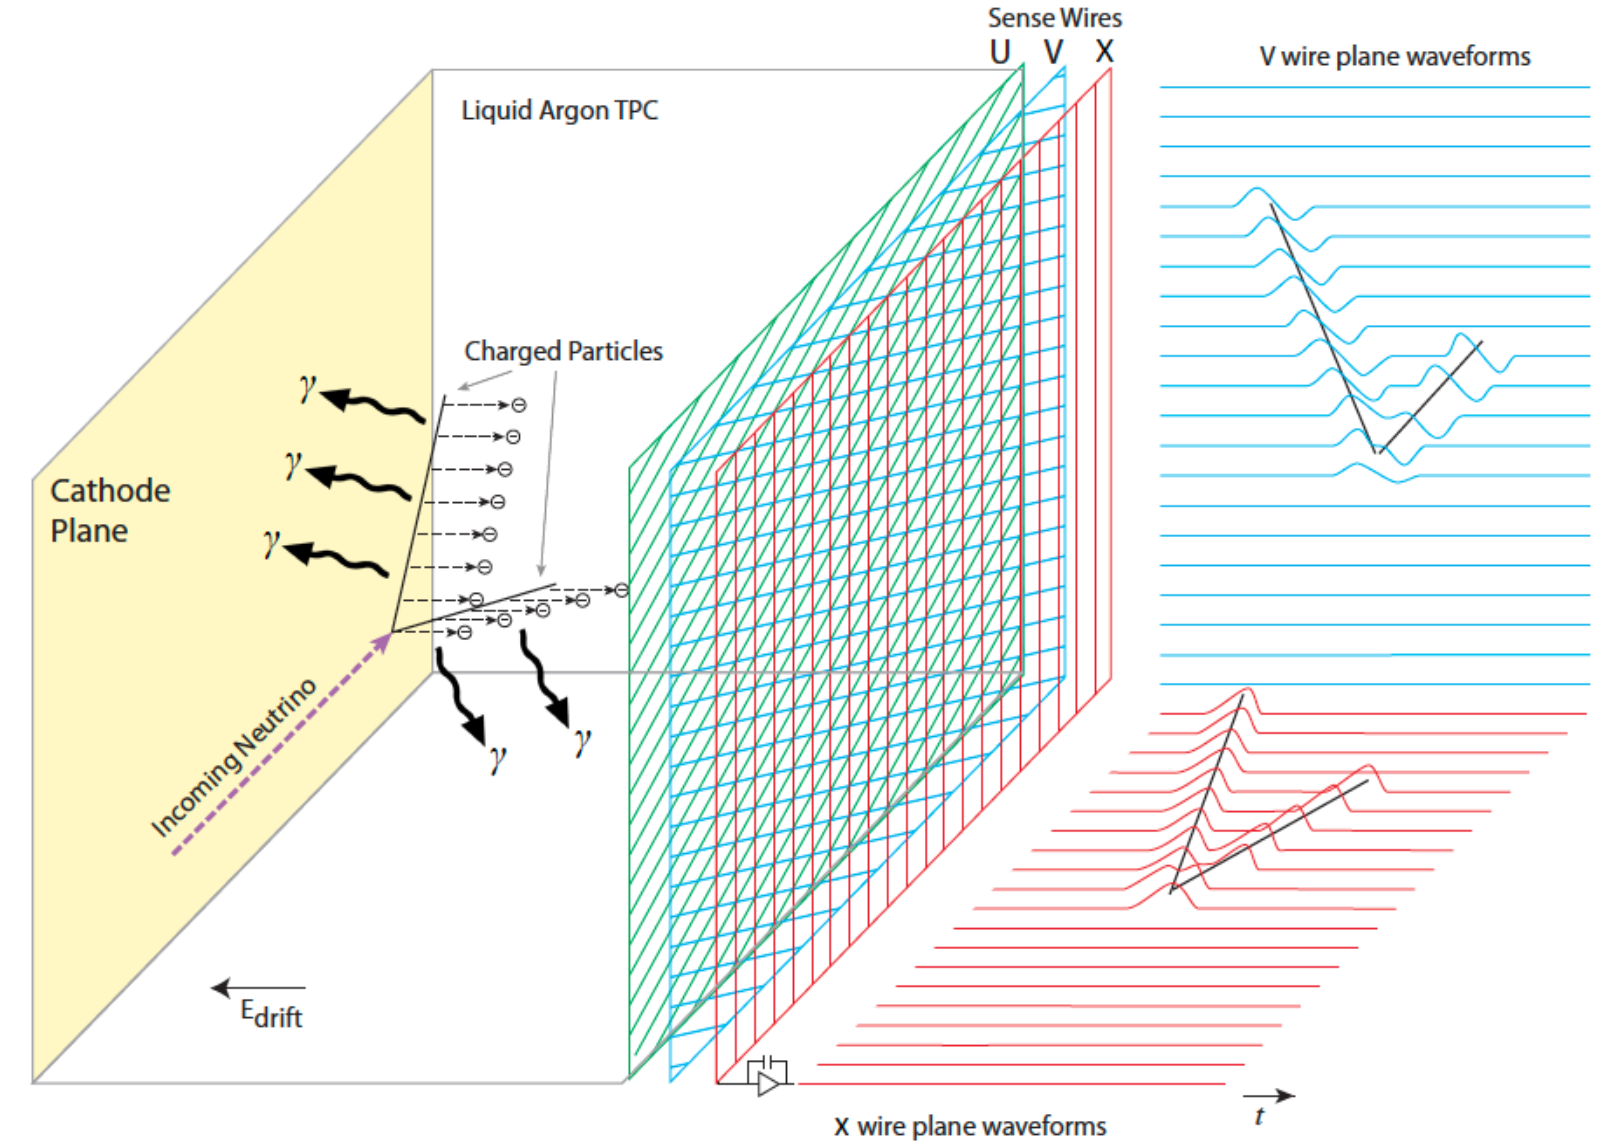
\includegraphics[width=0.8\linewidth]{Images/DUNE/FD/tpc}
	\caption[Schematic diagram showing the operating principle of a \gls{lartpc} with wire readout.]{Schematic diagram showing the operating principle of a \gls{lartpc} with wire readout. Figure taken from Ref. \cite{DUNE2020TDR1}.}
	\label{fig:lartpc}
\end{figure}

The \gls{dune} \gls{fd} complex will sit $1300~\mathrm{km}$ away from the beam target and $1.5~\mathrm{km}$ underground at \gls{surf}, South Dakota. Two caverns will host the four \gls{fd} modules, two of them per cavern, each embedded in cryostats of dimensions $18.9~\mathrm{m} ~ (\text{w}) \times 17.8~\mathrm{m} ~ (\text{h}) \times 65.8~\mathrm{m} ~ (\text{l})$. A central, smaller cavern will host the cryogenic system.

Three out of the four modules are confirmed to be \gls{lartpc} detectors, with a \gls{lar} fiducial mass of at least $10 ~ \mathrm{kt}$ each. The first and third \gls{fd} modules, \gls{fd}-1 and \gls{fd}-3, will use a Vertical Drift (\gls{vd}) technology, whereas the second module, \gls{fd}-2, will have a Horizontal Drift (\gls{hd}) direction. The technology for the fourth module is still to be decided. Detailed descriptions of the \gls{hd} and \gls{vd} designs can be found in the \gls{dune} \gls{fd} \gls{tdr} Volume IV \cite{DUNE2020TDR4} and the \gls{dune} \gls{fd} \gls{vd} \gls{tdr} \cite{DUNEVDTDR}, respectively.

For each event, with energies ranging from a few $\mathrm{MeV}$ to several $\mathrm{GeV}$, these detectors collect both the scintillation light and the ionisation electrons created when the charged particles produced in the neutrino-nucleus interactions ionise the argon nuclei. In both \gls{hd} and \gls{vd} designs the characteristic $128~\mathrm{nm}$ scintillation light of argon is collected by a photon detection system (\gls{pds}). This light will indicate the time at which electrons start to drift, thus enabling reconstruction over the drift coordinate when compared to the time when the first ionisation electrons arrive to the anode. Reconstruction of the topology in the transverse direction is achieved using the charge readout. Fig. \ref{fig:lartpc} illustrates the detection principle described, for the case of a \gls{hd} detector with a wire readout.

\subsection{Horizontal Drift}

\begin{figure}[t]
	\centering
	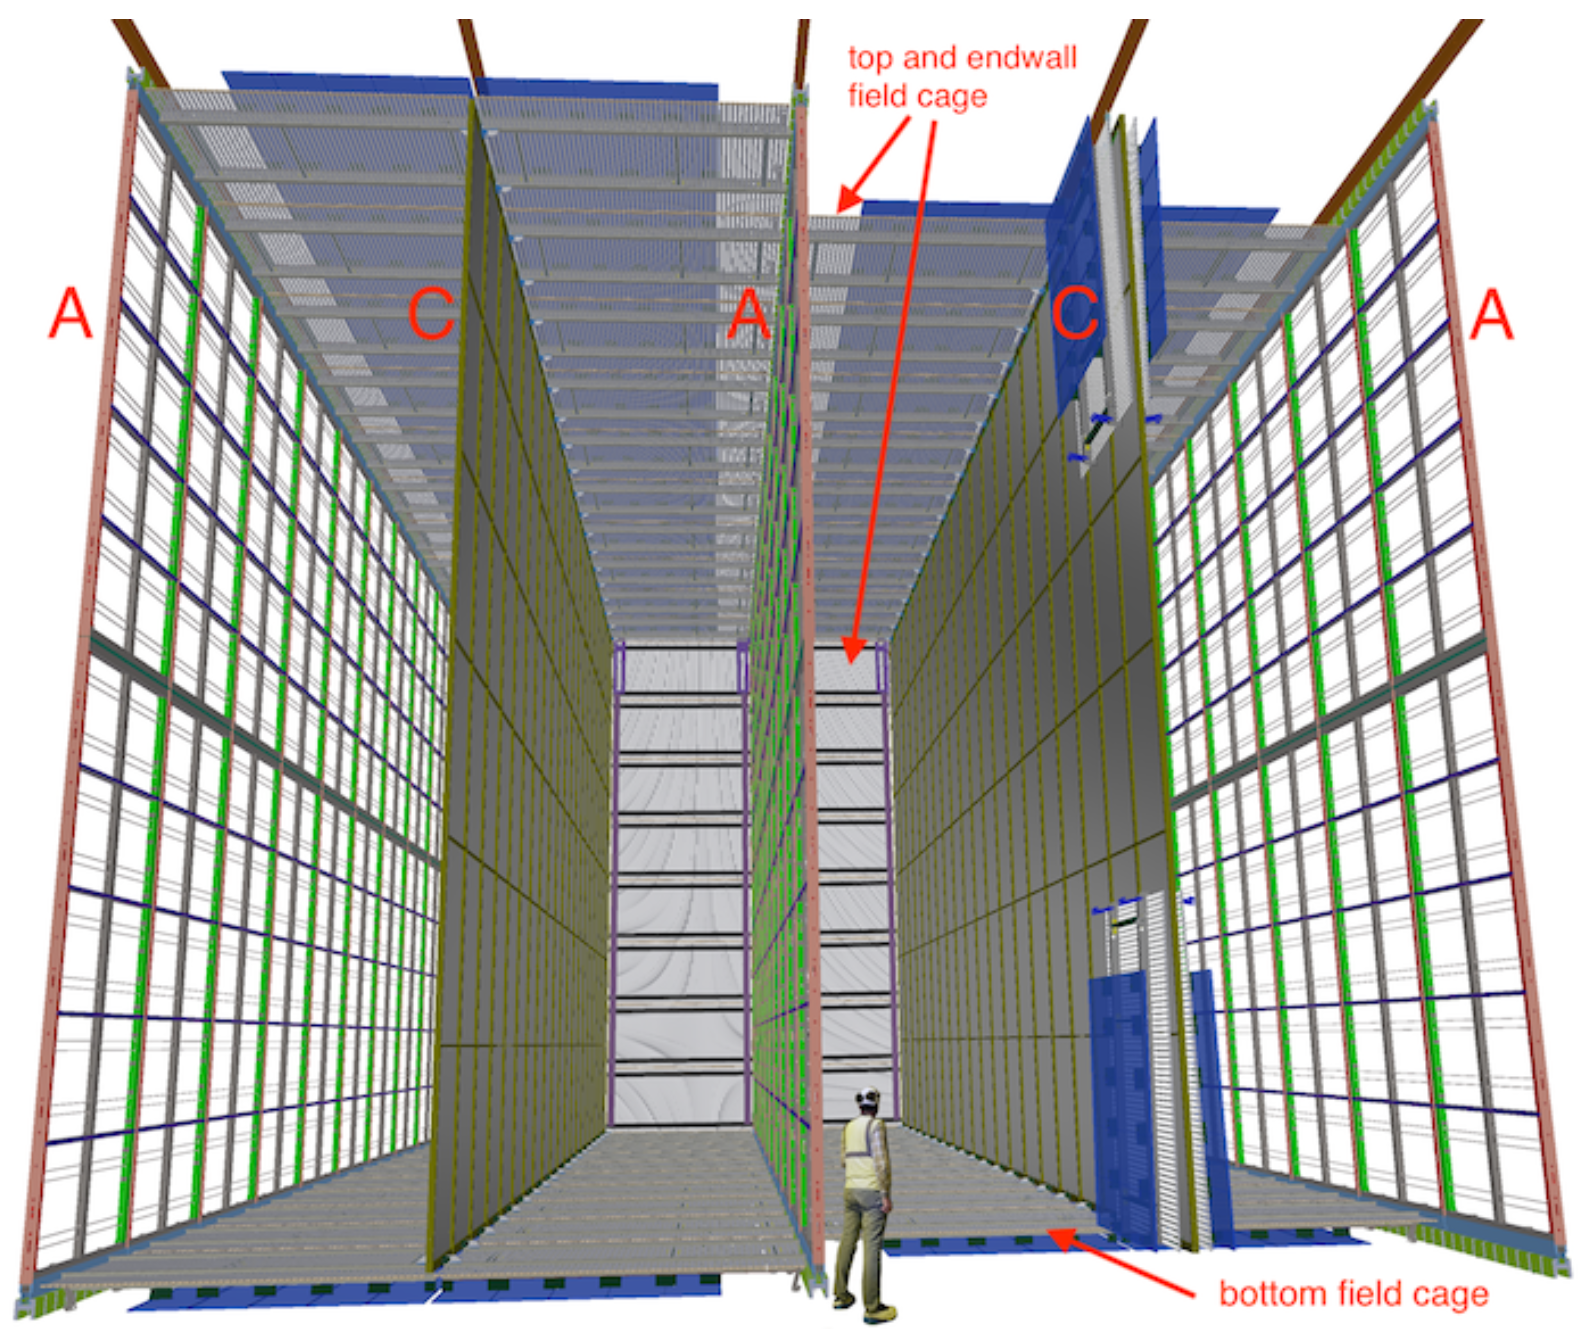
\includegraphics[width=0.65\linewidth]{Images/DUNE/FD/dune_hd}
	\caption[Proposed design for the \gls{fd}-2 module following the \gls{hd} principle.]{Proposed design for the \gls{fd}-2 module following the \gls{hd} principle. The labels A and C denote the anode and cathode walls, respectively. Figure taken from Ref. \cite{DUNE2020TDR1}.}
	\label{fig:dune_hd}
\end{figure}

In the \gls{hd} design the ionisation electrons produced as charged particles traverse the \gls{lar} drift horizontally towards the anode planes, due to the effect of an electric field. These anode planes are made out of three layers of wire readout. This design, previously known as single-phase (\gls{sp}), was tested in the ProtoDUNE-\gls{sp} detector at CERN. The prototype collected data from a hadron beam and cosmic rays, providing high-quality data sets for calibration and performance studies.

Each \gls{fd} \gls{hd} detector module is divided in four drift regions, with a maximum drift length of $3.5~\mathrm{m}$, by alternating anode and cathode walls. The surrounding field cage ensures the uniformity of the $500~\mathrm{V/cm}$ horizontal electric field across the drift volumes. The three anode walls, which constitute the charge readout of the detector, are built by stacking anode plane assemblies (\gls{apa}), 2 high times 25 wide. The design of the \gls{hd} modules is shown in Fig. \ref{fig:dune_hd}.

Each \gls{apa} is made of 2560 active wires arranged in three layers, plus an extra grid layer, wrapped around a metal frame. The two induction wire planes, U and V, sit at $\pm 35.7^{\circ}$ to the vertical on each side of the \gls{apa}. The collection and shielding plane wires, X and G, run parallel to the vertical direction. The ionisation electrons drift past the induction planes, generating bipolar signals on those wires, and are collected by the collection plane, producing a monopolar positive signal. The spacing between the wires is $\sim 5~\mathrm{mm}$, and it defines the spatial resolution of the \gls{apa}.

\begin{figure}[t]
	\centering
	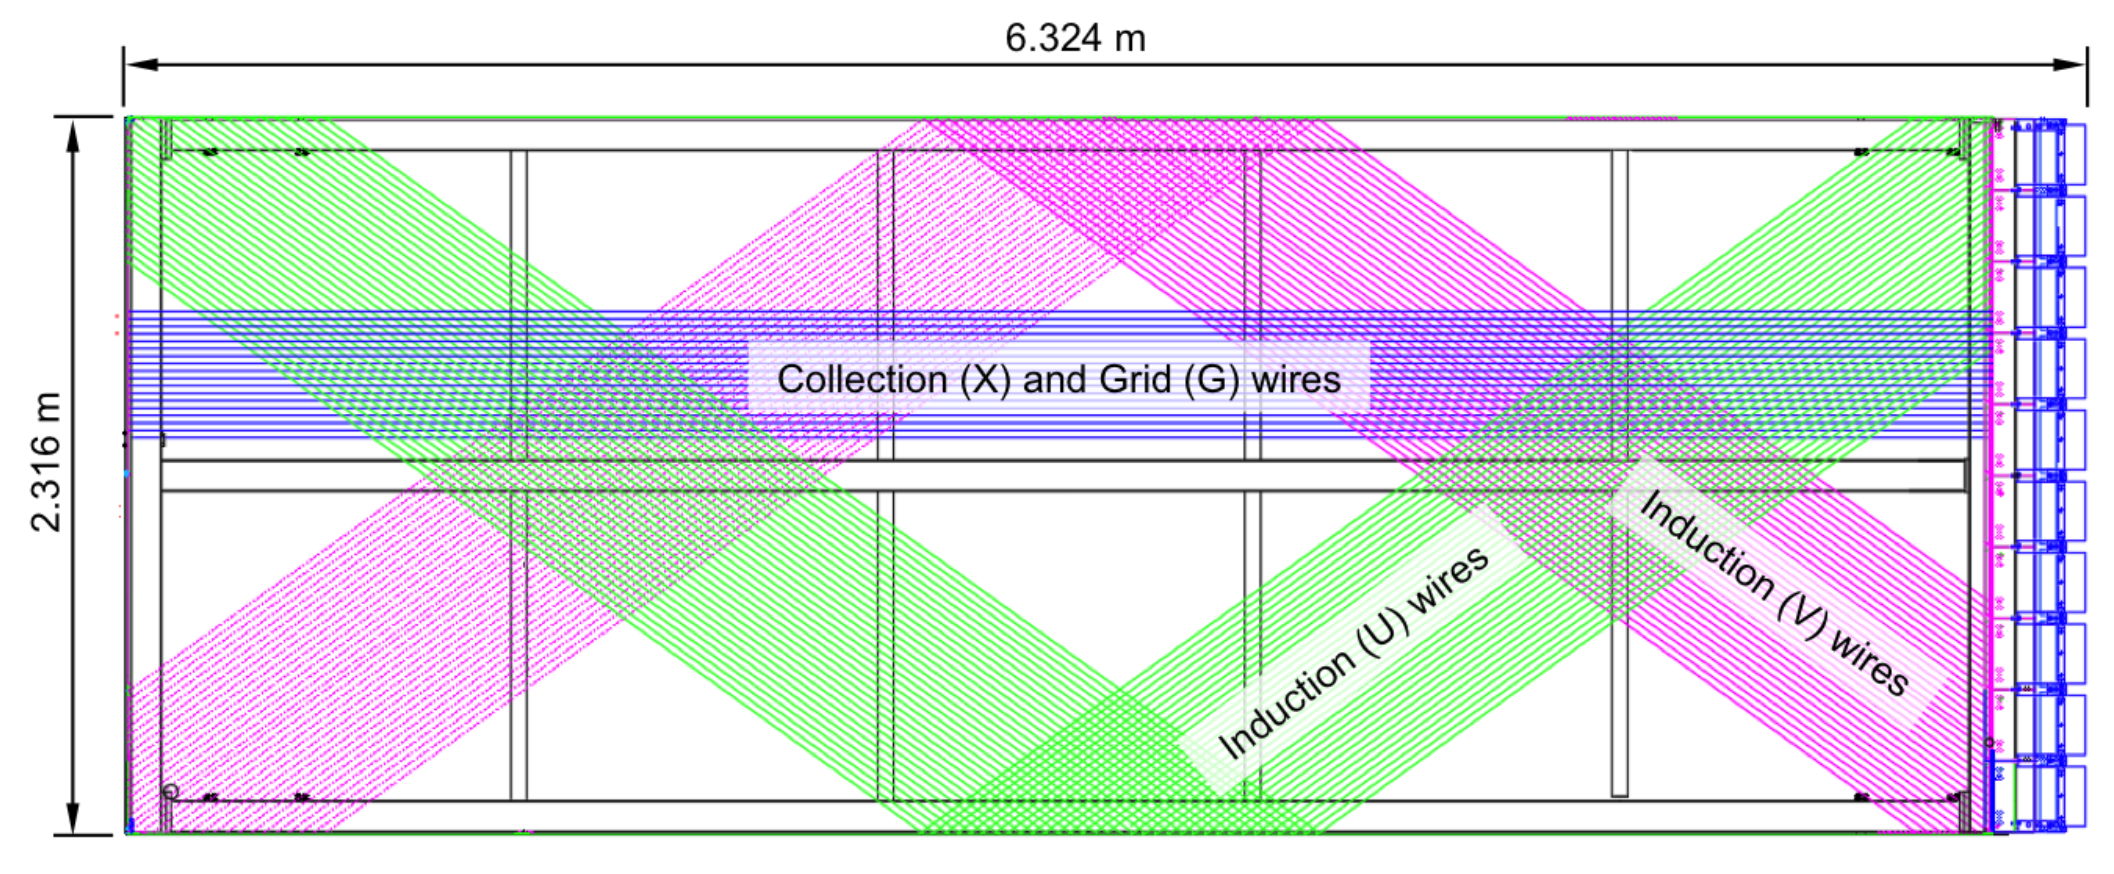
\includegraphics[width=1\linewidth]{Images/DUNE/FD/APA_wires}
	\caption[Schematic representation of an \gls{apa} frames showing the U, V, X and G wires.]{Schematic representation of an \gls{apa}. The black lines represent the \gls{apa} steel frame. The green and magenta lines correspond to the direction of the U and V induction wires respectively. The blue lines indicate the direction of the X collection wires and the wire shielding G. Figure taken from Ref. \cite{DUNE2020TDR1}.}
	\label{fig:apa}
\end{figure}

The front-end readout electronics, also called cold electronics as they are immersed in the \gls{lar}, are attached to the top of the up \gls{apa}s and the bottom of the down \gls{apa}s. Mounted on the front-end mother boards we have a series of \gls{asic}s that digitise the signals from the collection and induction planes. Each wire signal goes to a charge-sensitive amplifier, then to a pulse-shaping circuit, and finally to the analogue-to-digital converter. This part of the process happens inside the \gls{lar} to minimise the number of cables penetrating the cryostat. The digitised signals come out finally via a series of high-speed serial links to the warm interface boards (\gls{wib}s), from where the data is sent to the back-end \gls{daq} through optical fibers.

\begin{figure}[t]
	\begin{subfigure}{0.49\textwidth}
		\centering
		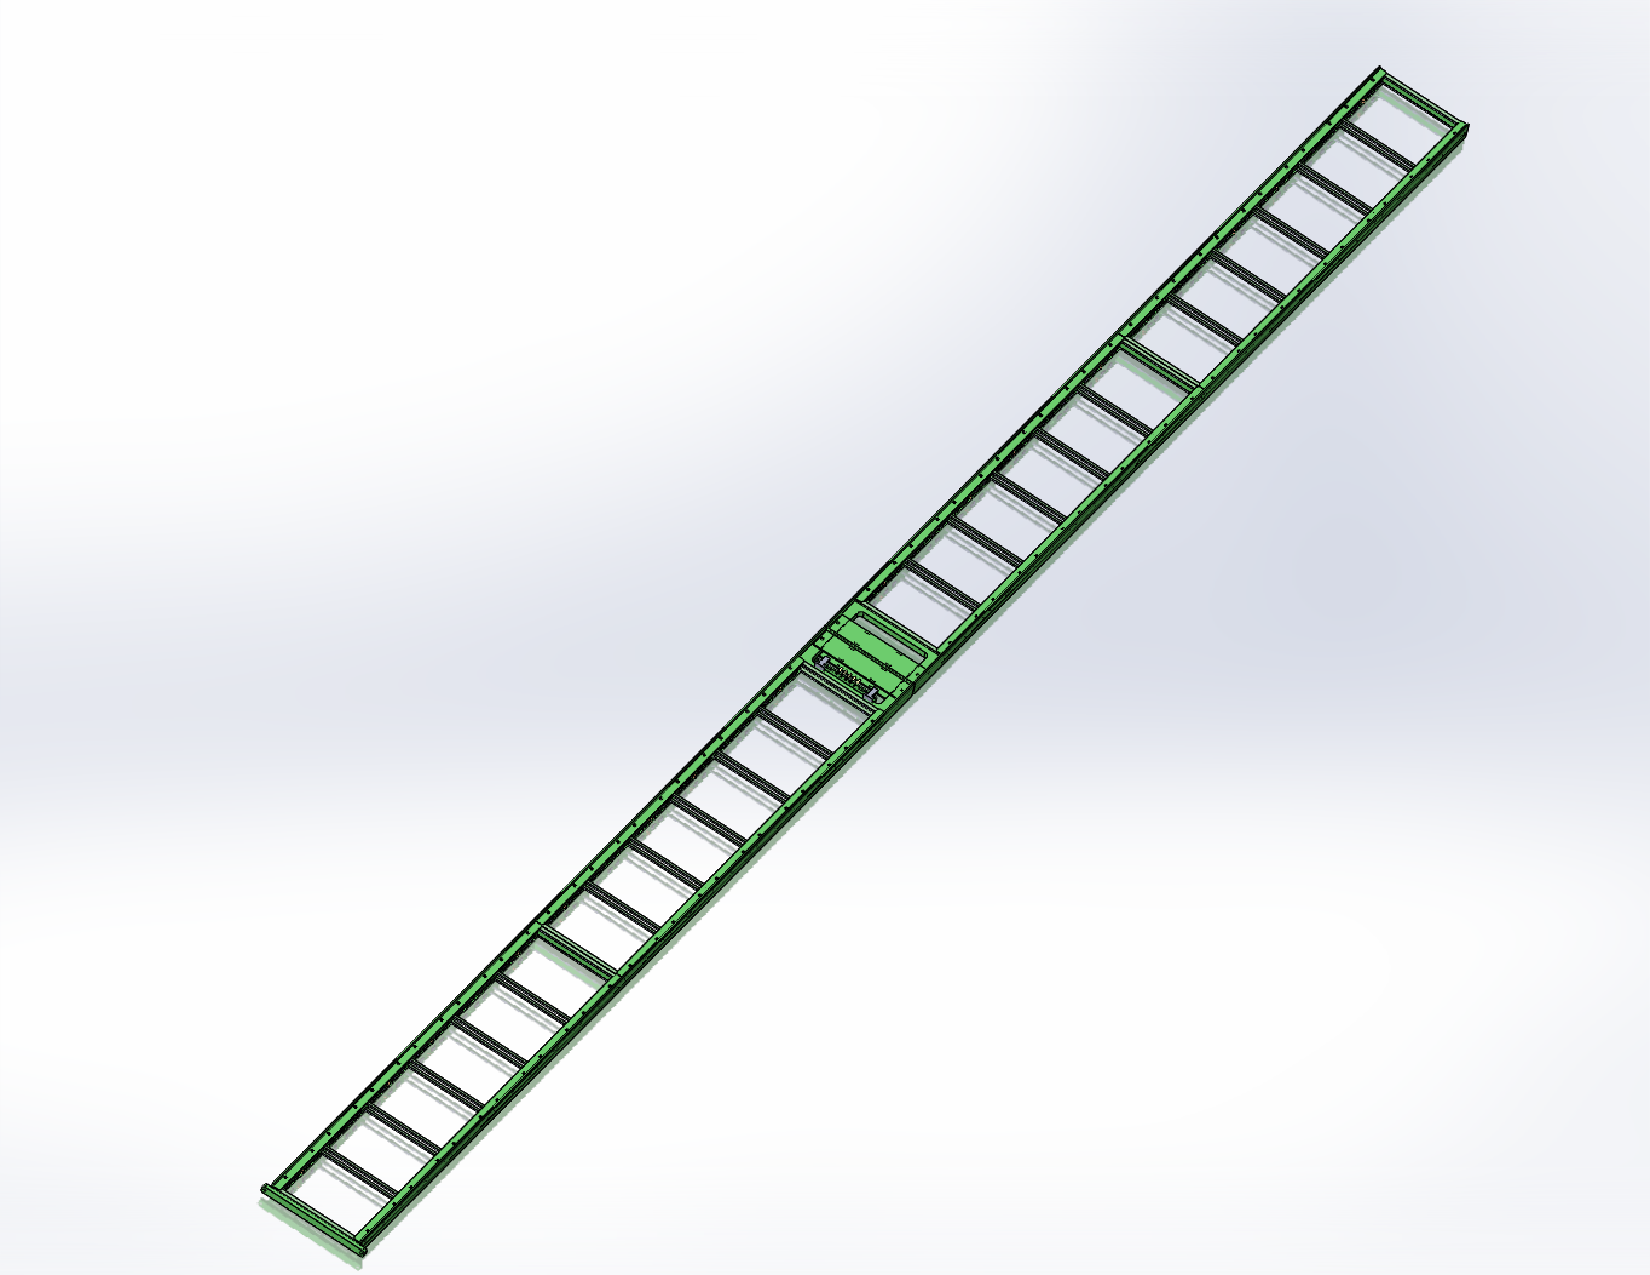
\includegraphics[width=.90\linewidth]{Images/DUNE/FD/pds-module}
	\end{subfigure}
	\begin{subfigure}{0.49\textwidth}
		\centering
		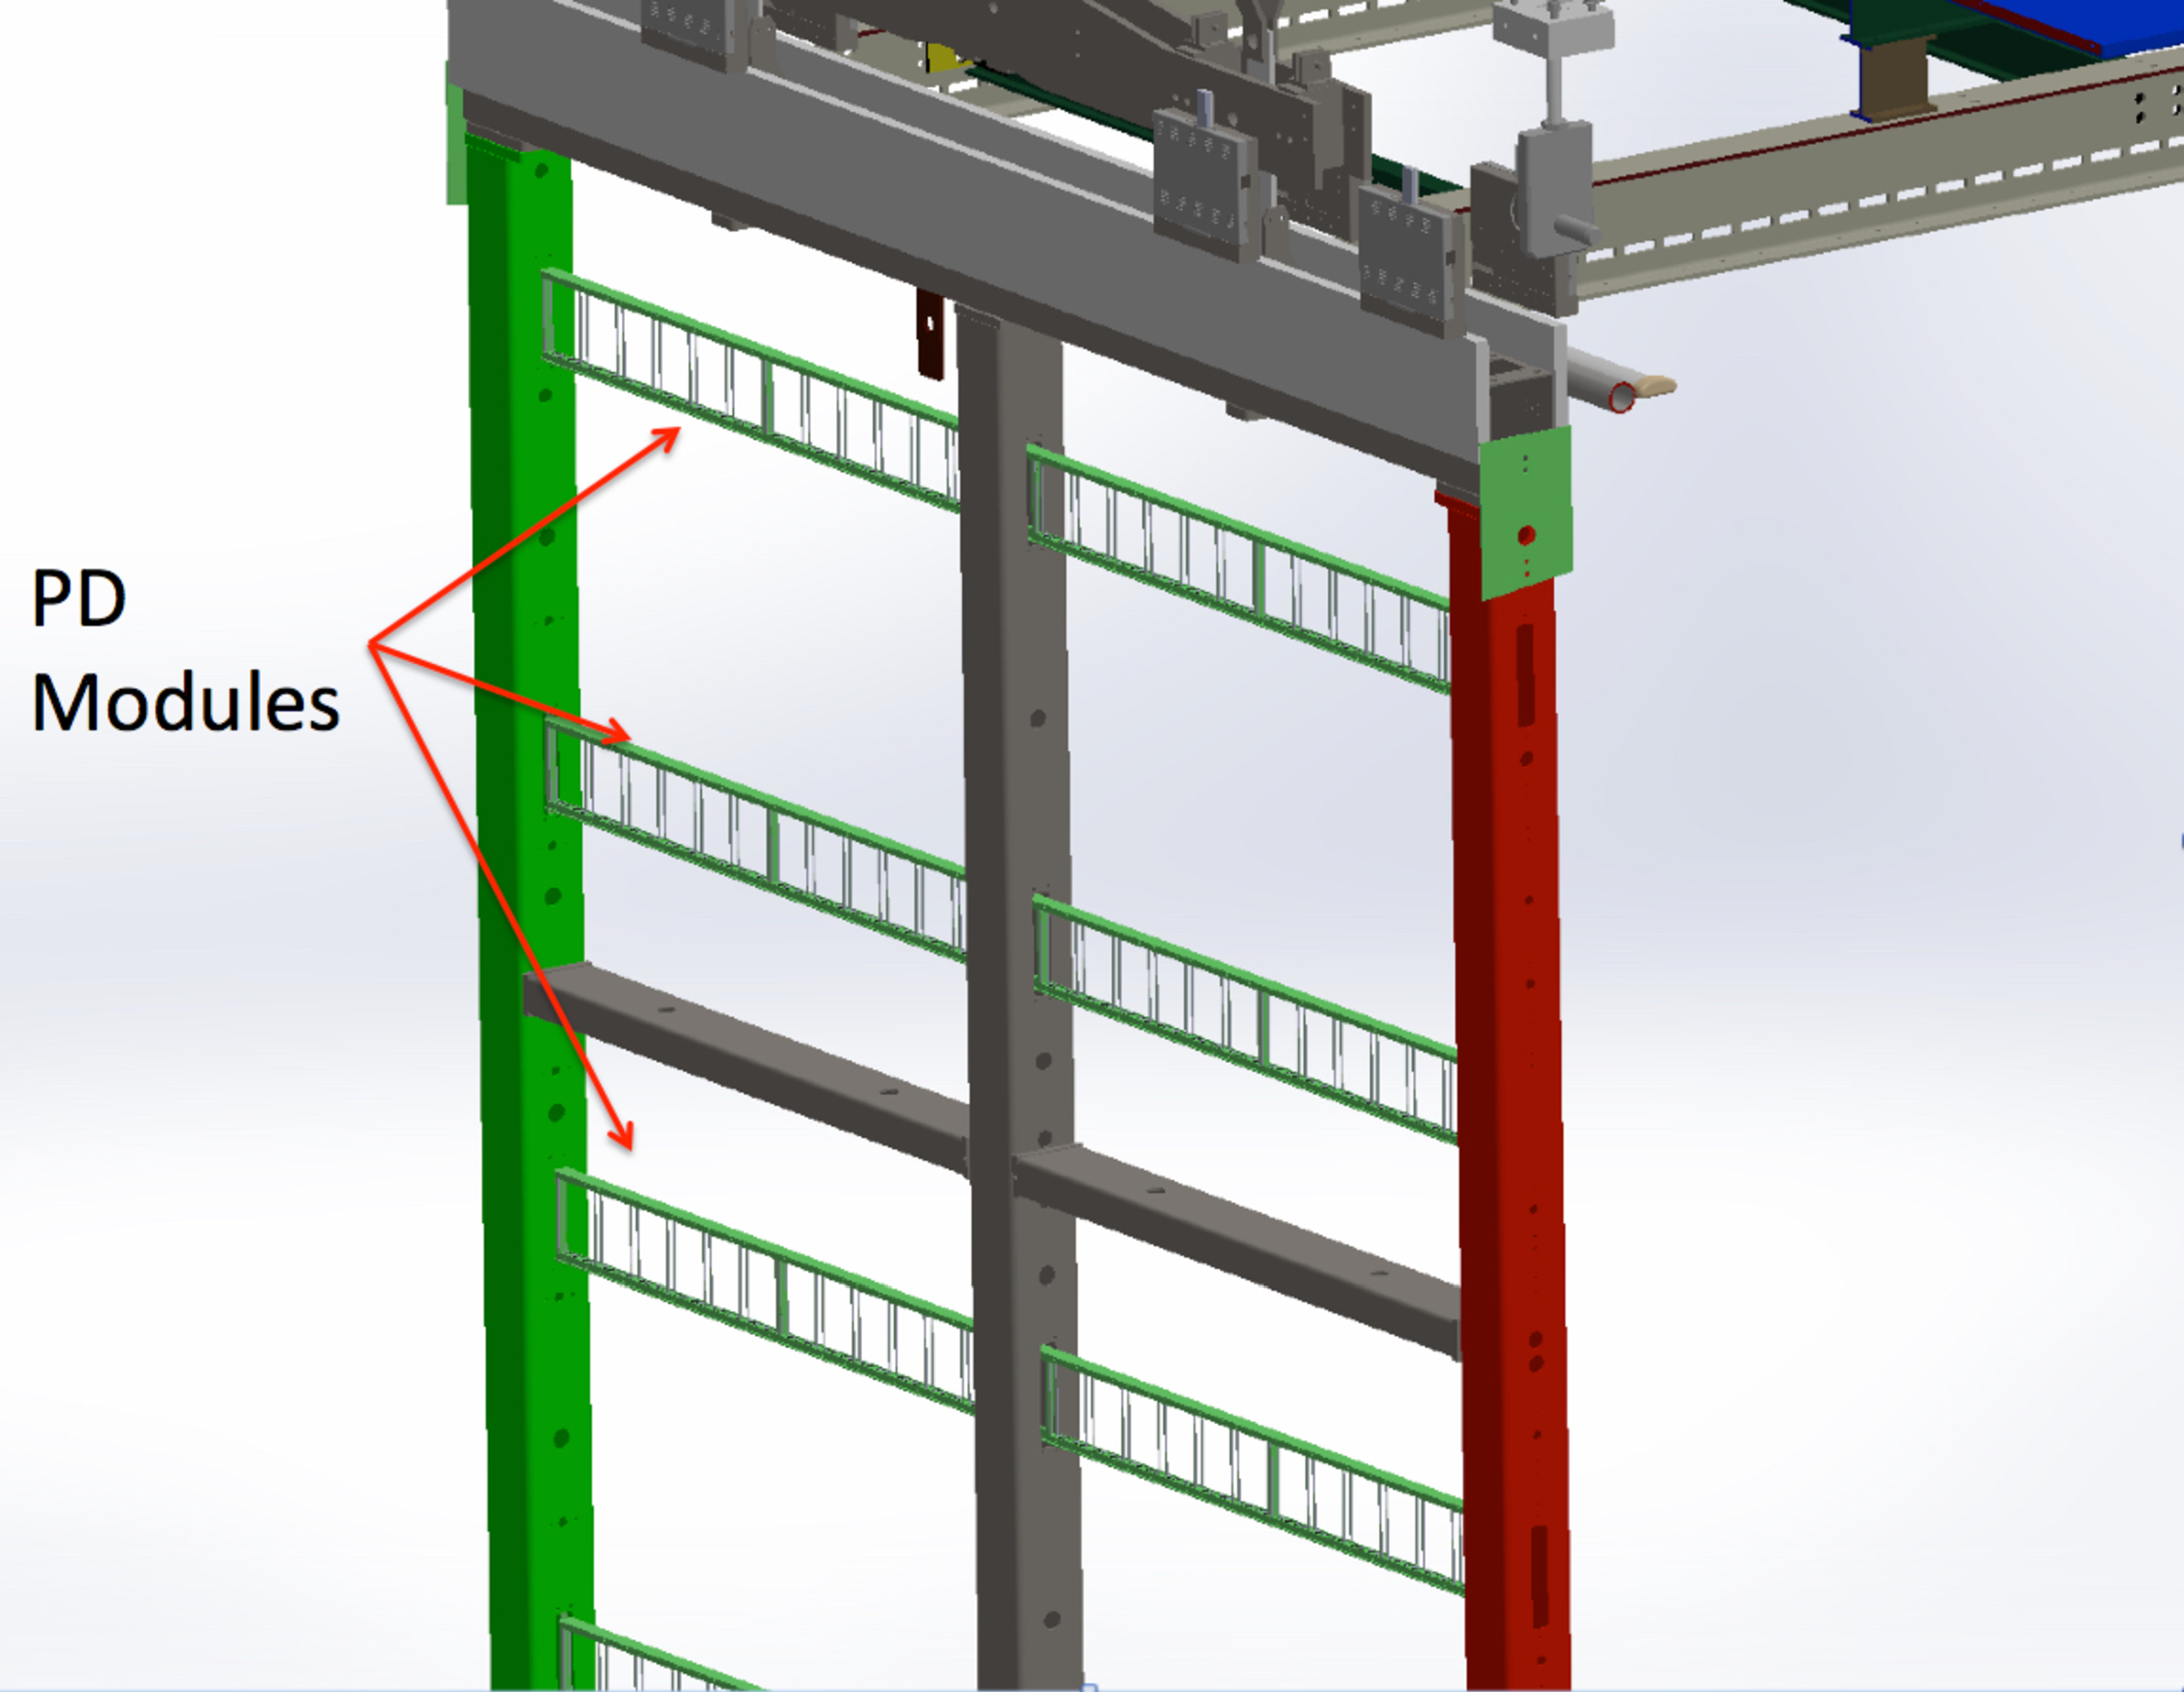
\includegraphics[width=.90\linewidth]{Images/DUNE/FD/pds-in-apa-assembly}
	\end{subfigure}
	\caption[A \gls{pds} module containing 24 X-ARAPUCAs and the location of the modules on the \gls{apa} frames.]{A \gls{pds} module containing 24 X-ARAPUCAs (left) and the location of the modules on the \gls{apa} frames (right). Figure taken from Ref. \cite{DUNE2020TDR1}.}
	\label{fig:dune_pds}
\end{figure}

The \gls{pds} uses modules of X-ARAPUCA devices, mounted on the \gls{apa} frames between the wire planes. Each X-ARAPUCA consists of layers of dichroic filter and wavelength-shifter. They shift the \gls{vuv} scintillation light into the visible spectrum, sending the visible photons to \gls{sipm} devices. The \gls{pds} modules are $209~\mathrm{cm}\times12~\mathrm{cm}\times2~\mathrm{cm}$ bars, containing 24 X-ARAPUCAs. There are 10 of these \gls{pds} modules per \gls{apa}. Fig. \ref{fig:dune_pds} shows a \gls{pds} module (left) and the placement of the modules on the \gls{apa}s (right).

\begin{comment}
	When using a \gls{sp} \gls{lartpc} there is no electron amplification, thus low noise is required by CE to extract the signals from the wires with a minimum S/N. In the worst operating case (short drift electron lifetime $\tau = 3 \ \mathrm{ms}$ and $E_{drift} = 250 \ \mathrm{V/cm}$) at least $10^{4}$ electrons will arrive to the anode from a minimum ionizing particle (MIP) near the cathode (farthest possible distance). Requiring at most $10^{3}$ electrons of equivalent noise charge (ENC) we will have a S/N $~\sim10$ for the collection wires. In the induction wires it results in S/N $\sim 5$, because of the bipolar shape of the signal. Keeping noise low (improving S/N) is crucial to achieve the physics goals. It allows proper event reconstruction and expand the boundaries on low-energy phenomena (\gls{snb}, $^{39}$Ar calibrations, etc.). Noise also affect \gls{daq} bandwidth, and can be a problem for astrophysical measurements.
\end{comment}

\subsection{Vertical Drift}

\begin{figure}[t]
	\centering
	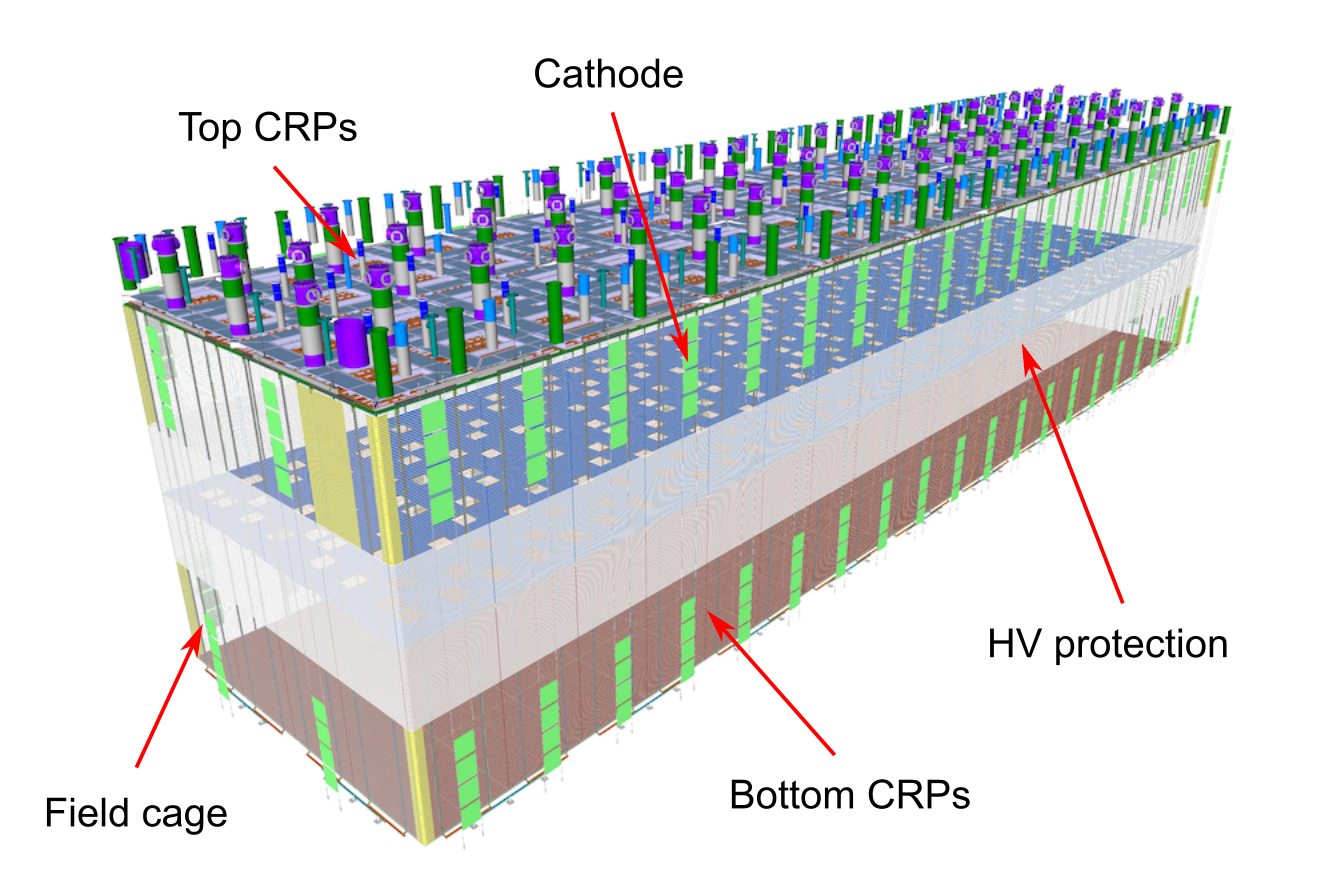
\includegraphics[width=0.70\linewidth]{Images/DUNE/FD/dune_vd}
	\caption[Proposed design for the \gls{fd}-1 and \gls{fd}-3 modules following the \gls{vd} principle.]{Proposed design for the \gls{fd}-1 and \gls{fd}-3 modules following the \gls{vd} principle. Figure adapted from Ref. \cite{DUNEVDTDR}.}
	\label{fig:dune_vd}
\end{figure}

In the \gls{vd} case the ionisation electrons will drift vertically until they meet a printed circuit board-based (\gls{pcb}) readout plane. It is based on the original dual-phase (\gls{dp}) design deployed at CERN, in the detector known as ProtoDUNE-\gls{dp}, which used a vertical drift design with an additional amplification of the ionisation electrons using a \gls{gar} layer above the liquid phase. The \gls{vd} module incorporates the positive features of the \gls{dp} design without the complications of having the \gls{lar}-\gls{gar} interface.

The current design of the \gls{fd} \gls{vd} module consists of two drift chambers with a maximum drift distance of $6.5~\mathrm{m}$. A cathode plane splits the detector volume perpendicular to the drift direction, while the two anode planes are connected to the bottom and top walls of the detector. The layout of a \gls{vd} module is shown in Fig. \ref{fig:dune_vd}. Compared with the \gls{hd} design, the \gls{vd} option offers a slightly larger instrumented volume and a more cost-effective solution for the charge readout.

\begin{figure}[t]
	\centering
	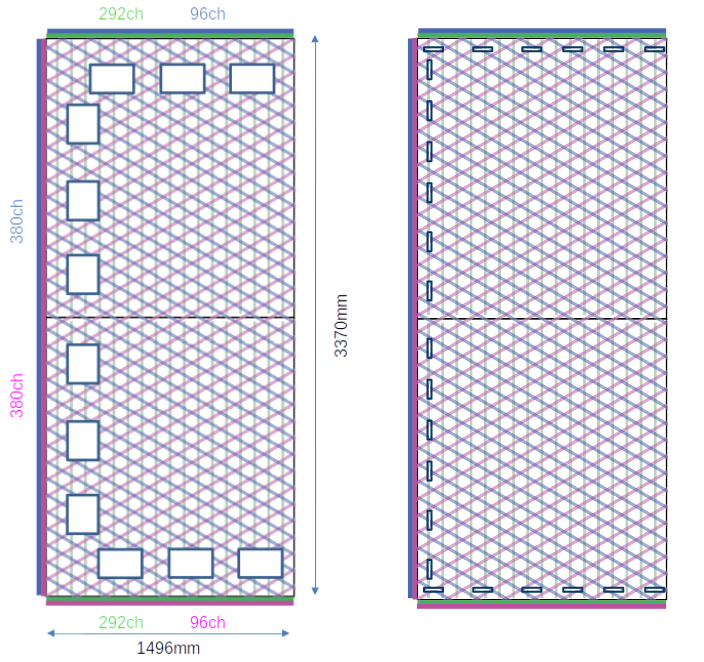
\includegraphics[width=0.70\linewidth]{Images/DUNE/FD/3V_anode_layout}
	\caption[Schematic representation of the electrode strip configuration for a top and bottom \gls{cru}.]{Schematic representation of the electrode strip configuration for a top (left) and bottom (right) \gls{cru}. Figure taken from Ref. \cite{DUNEVDTDR}.}
	\label{fig:dune_cru}
\end{figure}

As in the \gls{hd} design, each drift volume features a $500~\mathrm{V/cm}$ electric field and a field cage that ensures its uniformity. The anode planes are arrays of $3.4~\mathrm{m}\times3~\mathrm{m}$ charge-readout planes (\gls{crp}s). These are formed by a pair of charge-readout units (\gls{cru}s), which are built from two double-sided perforated \gls{pcb}s, with their perforations aligned. The perforations allow the drift electrons to pass between the layers.

The \gls{pcb} face opposite to the cathode has a copper guard plane which acts as shielding, while its reverse face is etched with electrode strips forming the first induction plane. The outer \gls{pcb} has electrode strips on both faces, the ones facing the inner \gls{pcb} form the second induction plane, while the outermost ones form the collection plane. Fig. \ref{fig:dune_cru} shows the layout of the electrode strips for the top (left) and bottom (right) \gls{cru}s. The magenta and blue lines represent the first and second induction planes, respectively, and the green lines correspond to the collection plane.

The \gls{pds} in the \gls{vd} module will use the same X-ARAPUCA technology developed for the \gls{hd} design. The plan is to place the \gls{pds} modules on the cryostat walls and on the cathode, in order to maximise the photon yield.

%\subsection{Module of opportunity}

\begin{figure}[t]
	\centering
	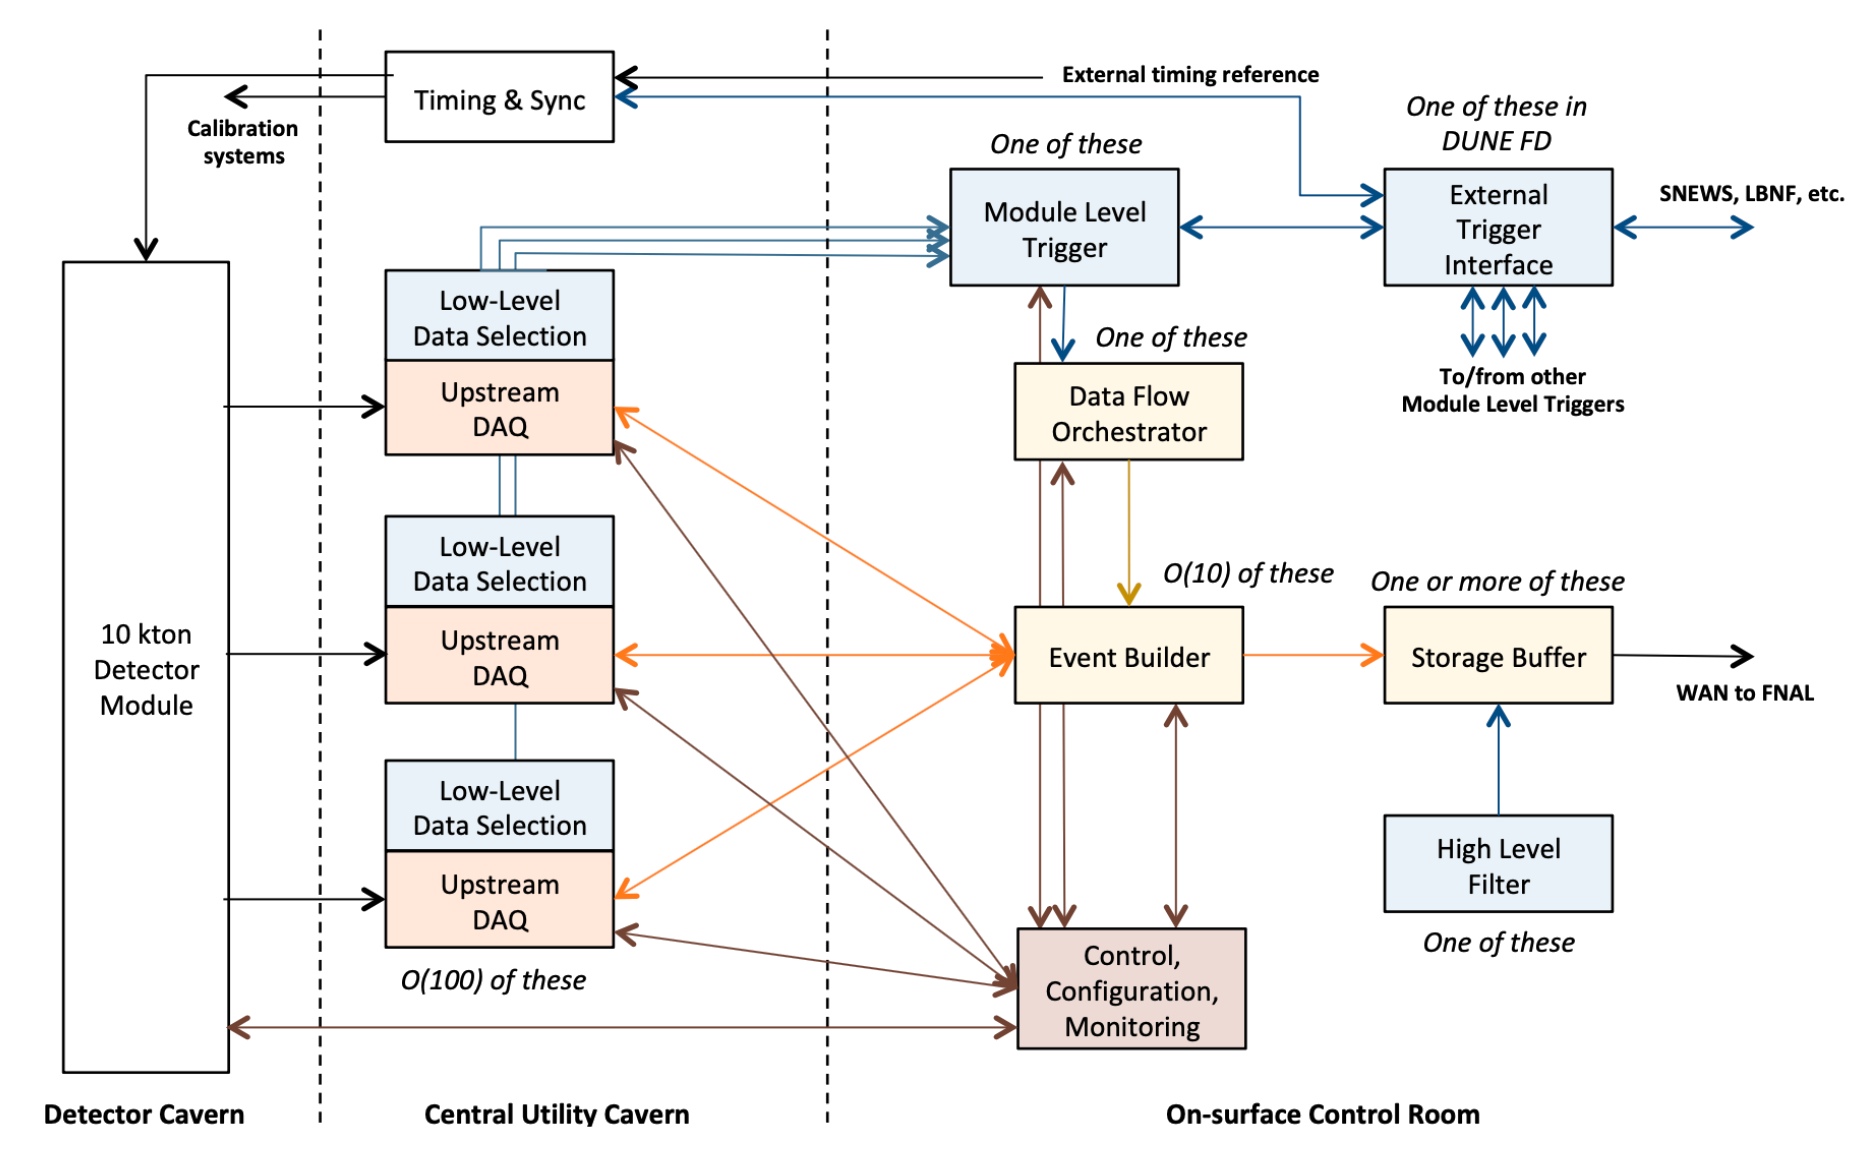
\includegraphics[width=0.8\linewidth]{Images/DUNE/FD/DAQ_detailed2}
	\caption[Detailed diagram of the \gls{dune} \gls{fd} \gls{daq} system.]{Detailed diagram of the \gls{dune} \gls{fd} \gls{daq} system. Figure taken from Ref. \cite{DUNE2020TDR4}.}
	\label{fig:daq1}
\end{figure}

\subsection{FD Data Acquisition System}

The data acquisition (\gls{daq}) system receives, processes and stores data from the detector modules. In the case of \gls{dune}, the \gls{daq} architecture is designed to work for all \gls{fd} modules interchangeably, except some aspects of the upstream part which may depend on the specific module technology.

The enormous sample rate and the number of channels in the \gls{tpc} and \gls{pds} readouts will produce a very large volume of data. These pose really strong requirements and challenges to the \gls{dune} \gls{fd} \gls{daq} architecture. It will be required to read out data of the order of ten thousand or more channels at rates of a few MHz. To cope with the huge data volume, segmented readouts and compression algorithms are used to reduce the data rate to manageable levels.

The \gls{daq} system of the \gls{dune} \gls{fd} is composed of five different subsystems. The first one is the upstream \gls{daq}, which receives the raw data from the detector, buffers it and performs some low-level pre-processing. The minimally processed data is then fed into a hierarchical data selection system, which then performs a module level trigger decision. In case of a positive decision, a trigger command is produced and executed by the data flow orchestrator, located in the back-end (\gls{be}) \gls{daq} subsystem. Subsequently, the \gls{daq} \gls{be} retrieves the relevant data from the buffers located in the upstream \gls{daq}, adds all the data into a cohesive record, and saves it to permanent storage. Watching over all the other subsystems we also have the control, configuration and monitoring subsystem and the time and synchronization subsystem. Figure \ref{fig:daq1} shows a schematic diagram of the \gls{daq} system, showing the different subsystems and their relations.

A notorious challenge for the \gls{dune} \gls{daq} system comes from its broad physics goals. We must be prepared to process events spanning a wide range of time windows, from $5 \ \mathrm{ms}$ in the case of beam and cosmic neutrinos and nucleon decay events, to $100 \ \mathrm{s}$ in the case of \gls{snb}s. This requires a continuous readout of the detector modules. Moreover, because of the off-beam measurements, we need to ensure the capabilities of online data processing and self-triggering. Taking this into account, together with the technical constraints, the \gls{dune} \gls{fd} \gls{daq} faces a series of challenges: it needs to be fault tolerant and redundant to reduce downtime, accommodate new components while it keeps serving the operational modules, have large upstream buffers to handle \gls{snb} physics, be able to support a wide range of readout windows, and reduce the throughput of data to permanent storage to be at most $30 \ \mathrm{PB/year}$.